\documentclass[man]{apa6}
\usepackage{lmodern}
\usepackage{amssymb,amsmath}
\usepackage{ifxetex,ifluatex}
\usepackage{fixltx2e} % provides \textsubscript
\ifnum 0\ifxetex 1\fi\ifluatex 1\fi=0 % if pdftex
  \usepackage[T1]{fontenc}
  \usepackage[utf8]{inputenc}
\else % if luatex or xelatex
  \ifxetex
    \usepackage{mathspec}
  \else
    \usepackage{fontspec}
  \fi
  \defaultfontfeatures{Ligatures=TeX,Scale=MatchLowercase}
\fi
% use upquote if available, for straight quotes in verbatim environments
\IfFileExists{upquote.sty}{\usepackage{upquote}}{}
% use microtype if available
\IfFileExists{microtype.sty}{%
\usepackage{microtype}
\UseMicrotypeSet[protrusion]{basicmath} % disable protrusion for tt fonts
}{}
\usepackage{hyperref}
\hypersetup{unicode=true,
            pdftitle={The Emotion--Facial expression link: Evidence from Human and Automatic Expression Recognition},
            pdfauthor={Anna Tcherkassof~\& Damien Dupré},
            pdfkeywords={Facial expression, self-report, human observer, automatic recognition.},
            pdfborder={0 0 0},
            breaklinks=true}
\urlstyle{same}  % don't use monospace font for urls
\usepackage{longtable,booktabs}
\usepackage{graphicx,grffile}
\makeatletter
\def\maxwidth{\ifdim\Gin@nat@width>\linewidth\linewidth\else\Gin@nat@width\fi}
\def\maxheight{\ifdim\Gin@nat@height>\textheight\textheight\else\Gin@nat@height\fi}
\makeatother
% Scale images if necessary, so that they will not overflow the page
% margins by default, and it is still possible to overwrite the defaults
% using explicit options in \includegraphics[width, height, ...]{}
\setkeys{Gin}{width=\maxwidth,height=\maxheight,keepaspectratio}
\IfFileExists{parskip.sty}{%
\usepackage{parskip}
}{% else
\setlength{\parindent}{0pt}
\setlength{\parskip}{6pt plus 2pt minus 1pt}
}
\setlength{\emergencystretch}{3em}  % prevent overfull lines
\providecommand{\tightlist}{%
  \setlength{\itemsep}{0pt}\setlength{\parskip}{0pt}}
\setcounter{secnumdepth}{5}
% Redefines (sub)paragraphs to behave more like sections
\ifx\paragraph\undefined\else
\let\oldparagraph\paragraph
\renewcommand{\paragraph}[1]{\oldparagraph{#1}\mbox{}}
\fi
\ifx\subparagraph\undefined\else
\let\oldsubparagraph\subparagraph
\renewcommand{\subparagraph}[1]{\oldsubparagraph{#1}\mbox{}}
\fi

%%% Use protect on footnotes to avoid problems with footnotes in titles
\let\rmarkdownfootnote\footnote%
\def\footnote{\protect\rmarkdownfootnote}


  \title{The Emotion--Facial expression link: Evidence from Human and Automatic Expression Recognition}
    \author{Anna Tcherkassof\textsuperscript{1}~\& Damien Dupré\textsuperscript{2}}
    \date{}
  
\shorttitle{The Emotion–Facial expression link}
\affiliation{
\vspace{0.5cm}
\textsuperscript{1} University Grenoble Alpes, Grenoble, France\\\textsuperscript{2} Dublin City University, Dublin, Ireland}
\keywords{Facial expression, self-report, human observer, automatic recognition.\newline\indent Word count: 7998}
\usepackage{csquotes}
\usepackage{upgreek}
\captionsetup{font=singlespacing,justification=justified}

\usepackage{longtable}
\usepackage{lscape}
\usepackage{multirow}
\usepackage{tabularx}
\usepackage[flushleft]{threeparttable}
\usepackage{threeparttablex}

\newenvironment{lltable}{\begin{landscape}\begin{center}\begin{ThreePartTable}}{\end{ThreePartTable}\end{center}\end{landscape}}

\makeatletter
\newcommand\LastLTentrywidth{1em}
\newlength\longtablewidth
\setlength{\longtablewidth}{1in}
\newcommand{\getlongtablewidth}{\begingroup \ifcsname LT@\roman{LT@tables}\endcsname \global\longtablewidth=0pt \renewcommand{\LT@entry}[2]{\global\advance\longtablewidth by ##2\relax\gdef\LastLTentrywidth{##2}}\@nameuse{LT@\roman{LT@tables}} \fi \endgroup}


\DeclareDelayedFloatFlavor{ThreePartTable}{table}
\DeclareDelayedFloatFlavor{lltable}{table}
\DeclareDelayedFloatFlavor*{longtable}{table}
\makeatletter
\renewcommand{\efloat@iwrite}[1]{\immediate\expandafter\protected@write\csname efloat@post#1\endcsname{}}
\makeatother
\usepackage{lineno}

\linenumbers
\usepackage{booktabs}
\usepackage{float}
\usepackage{tabu}
\usepackage{wrapfig}
\usepackage[none]{hyphenat}
\floatplacement{figure}{H}
\usepackage{flushend}
\usepackage{biblatex}

\authornote{

Correspondence concerning this article should be addressed to Anna Tcherkassof, Bâtiment Michel Dubois, Université Grenoble Alpes, 1251 Avenue Centrale, 38400 Saint-Martin-d'Hères. E-mail: \href{mailto:anna.tcherkassof@univ-grenoble-alpes.fr}{\nolinkurl{anna.tcherkassof@univ-grenoble-alpes.fr}}}

\abstract{
While it has been taken for granted in the development of several automatic facial expression recognition tools, the question of the coherence between subjective feelings and facial expressions is still a subject of debate. On one hand, the Basic Emotion View conceives emotions as genetically hardwired and therefore being genuinely displayed through facial expressions. On the other hand, the constructivist approach conceives emotions as socially constructed; the emotional meaning of a facial expression being inferred by the observer. In order to evaluate the coherence between the subjective feeling of emotions and their recognition based on facial expression, 232 videos of encoders recruited to carry out an emotion elicitation task were annotated by 1383 human observers as well as by an automatic facial expression classifier. Results show low accuracy of human observers and of the automatic classifier to infer the subjective feeling from the facial expressions displayed by encoders. They also show a weak consistency between self-reported emotional states and facial emotional displays. Based on these results, the hypothesis of genetically hardwired emotion genuinely displayed is difficult to support, whereas the idea of emotion and facial expression socially constructed appears to be more likely. Accordingly, automatic emotion recognition tools based on facial expressions should be questioned.


}

\begin{document}
\maketitle

{
\setcounter{tocdepth}{2}
\tableofcontents
}






\hypertarget{introduction}{%
\section{Introduction}\label{introduction}}

With the development of commercial automatic facial expression recognition tools (Dupré, Andelic, Morrison, \& McKeown, 2018), industries and governments are gradually implementing this technology in order to monitor humans' emotions in various scenarios (\emph{e.g.}, in marketing, healthcare, and the automotive industry to name a few). This technology rests on the premise that facial expressions provide a direct access to individuals' subjective feelings, and that one can read the emotions displayed on a person's face as in an open book. This premise is derived from the Basic Emotion View which suggests a one-to-one mapping between subective feeling and facial expression (Ekman, 1992, 2007; Ekman et al., 1987; Ekman \& Heider, 1988). Even if this premise is central to the modern mainstream approach of human emotion, recent research in affective science is challenging it. Once the Basic Emotion View is briefly described, its foremost criticisms are synthetically exposed. Inconsistencies and unpredicted findings research has uncovered come both from field observations and laboratory experiments. They relate to two different issues. The first issue is the one of the sender's production of spontaneous facial displays. The second issue has to do with the viewer's interpretation of these facial displays. Building on this evidence, and as a further attempt to shed light on the emotion--face link, the present study is finally exposed. Its main goal is to tackle these two issues at the same time. It aims at identifying the extent to which ordinary people's experienced emotions are displayed through identifiable emotional facial expressions (EFE) recognized as such both by human individuals and by automatic facial expression recognition tools.

\hypertarget{the-basic-emotion-view}{%
\subsection{The Basic Emotion View}\label{the-basic-emotion-view}}

The belief that facial expression is linked to emotional states can be traced back to Darwin in \emph{The Expression of the Emotions in Man and Animals} (Darwin, 1872). Countless studies have fortified the idea that emotional states are inherently coupled to a set of prototypic facial expressions (\emph{e.g.}, Ekman \& Cordaro, 2011). The Basic Emotion View holds that facial expressions are genuine displays of an individual's inner emotional state. More specifically, a set of six emotions (\emph{fear}, \emph{anger}, \emph{surprise}, \emph{disgust}, \emph{sadness} and \emph{joy}) are universally displayed and are genetically hardwired not only in humans (Ekman, 1992), but also in different animal species (Waal, 2019). According to the view of the Basic Emotion View, \emph{\enquote{when emotions are aroused by perception of a social event, a set of central commands produce patterned emotion-specific changes in multiple systems, including {[}\ldots{}{]} facial expressions.}} (Ekman, 2007, p. 49). To respond to criticisms, several amendments have been made to the Basic Emotion View, increasing the number of basic emotions from six to seven (Ekman \& Heider, 1988) as well as adding the concept of \enquote{display rules} to explain cultural differences in the management of facial expressions (Ekman et al., 1987).

Relatively few studies have actually tested Basic Emotion View's fundamental claim regarding the facial production (so-called \enquote{expression}) of emotions. Rosenberg \& Ekman (1994) reported the first evidence of coherence between self-report of emotion and displayed facial expressions. Participants were showed emotionally evocative films and reported their own emotions using a moment-by-moment reporting procedure. Analysis of participants' facial expressions and reports of emotions showed that there was a high degree of temporal linkage and emotional agreement between facial expressions and self-reports. Notwithstanding this study, few have used purely descriptive methods such as electromyography or objective face coding systems to identify and to measure the actual changes in the face when a given emotion is felt (see Wagner, 1997, for methodological points). Much of the research has focused instead on the recognition of EFE, that is on the issue of the viewer's interpretation of facial displays. As people have been thought to display their internal state, EFE supposedly serve as a window into the emotions of others. Viewers \enquote{recognize} the facial displays and infer the corresponding emotional state. The Readout Hypothesis (Buck, 1985) formalizes this folk theory. According to it, facial expressions have evolved to provide \emph{\enquote{an external readout of those motivational-emotional processes that have had social implications during the course of evolution}} (Buck, 1985, pp. 396--397). Thus, as readouts of emotional states, spontaneous expressive displays are directly accessible to other organisms. Research on the inference of emotions from facial expressions has established that viewers show considerable agreement that the so-called basic emotions---happiness, anger, fear, disgust, sadness, and surprise---are associated with specific facial displays (\emph{e.g.}, reviews from Elfenbein \& Ambady, 2002; Russell, 1994).

Yet, in spite of the popular support it has received, the empirical data called upon by the Basic Emotion View remains unpersuasive. Notably, it fails to explain, in instances in which display rules cannot be called upon, how individuals can feel emotions without expressing them or how individuals can express emotions without feeling them, and why observers are not totally accurate in recognizing facial expressions of basic emotions, among others. The following is a summary of key findings and conclusions both from field observations and laboratory experiments on spontaneous expression of emotions, all of them strongly subverting the Basic Emotion viewpoint (for reviews, Fernández-Dols \& Crivelli, 2013; Reisenzein, Studtmann, \& Horstmann, 2013; Russell, Bachorowski, \& Fernández-Dols, 2003). Mains issues regarding recognition studies are also swept across afterwards.

\hypertarget{spontaneous-facial-expression-in-naturalistic-studies}{%
\subsection{Spontaneous Facial Expression in naturalistic studies}\label{spontaneous-facial-expression-in-naturalistic-studies}}

Naturalistic studies look at the ecological frequency of co-occurrence of certain emotions and facial displays (Fernández-Dols \& Crivelli, 2013). Though they cannot be considered as a straightforward test of the triggering role of emotion on the facial behavior, they have the advantage of considering situations that cannot be created in a laboratory. For instance, the ethological study of Kraut \& Johnston (1979) contradicts the Basic Emotion View premise that a smile is the major component of a facial display associated with and caused by feelings of joy or happiness. Naturalistic observation at a bowling alley showed that bowlers do not necessarily smile after scoring a spare or a strike (a situation likely to elicit a positive emotion). Rather, they often smile when interacting with other people. More generally, examination of bowlers' facial display showed that they rarely smiled while facing the pins but often smiled when facing their friends. These findings were confirmed by Ruiz-Belda, Fernández-Dols, Carrera, \& Barchard (2003) who analyzed the facial displays of bowlers after a strike and soccer fans after their team scored. Their results show a low probability of smiling when participants were not interacting with someone else. These findings have been supported in other realistic field settings such as the one of Fernández-Dols \& Ruiz-Belda (1995) suggesting that happiness is not a sufficient cause of smiling. Fernández-Dols \& Ruiz-Belda (1995) watched extremely happy gold medalist athletes displaying facial expressions of sadness (sometimes associated with tears) during their Olympics awards ceremonies. More specifically, winners showed Duchenne smiles and other types of smiles when they were interacting with other people during the awards ceremony, but smiles were scarce or nonexistent when waiting behind the podium and/or when turning toward the flagpoles and focusing their attention on the flags and the national anthem. Crivelli, Carrera, \& Fernández-Dols (2015) also found that the strongest predictor for the occurrence of Duchenne smiles in judo winners is when they are engaged in social interaction and not when they just won their match.

Happiness/joy is not the only emotion weakly associated with the predicted facial expression. A naturalistic study conducted by Scherer \& Ceschi (1997) in an airport's baggage handling office showed that passengers claiming for their lost luggage displayed very few facial expressions of negative emotions while self-reporting subjective feeling states of anger or sadness among others. The covariation between passengers' self-ratings and the claims agents' attributions of the passengers' emotions was very low. Another refutation of the Basic Emotion View's predictions regarding the link between emotions and facial expressions is provided by naturalistic observations of infants' productions of facial expressions. It is often acknowledged that adults regulate their expressive behavior. In accordance with various display rules (personal, social, cultural ones), they exert a control over the supposed automatic readouts of their emotions. Developmental studies provide relevant settings in which display rules are inoperative. Camras and her colleagues observed that facial expressions of negative emotions were displayed in circumstances that were unlikely to have elicited those emotions. For instance, infants displayed \enquote{fear} expressions in settings not related to fear (Camras, Malatesta, \& Izard, 1991). Bennett, Bendersky, \& Lewis (2002) videotaped a sample of 4-month-old infants during tickle, sour taste, jack-in-the-box, arm restraint, and masked stranger situations. Infants displayed a variety of facial expressions in each eliciting situation. Yet, more infants exhibited positive than negative facial expressions across all situations --except sour taste. No evidence for emotion-specific facial expressions corresponding to anger, fear, and sadness was obtained. Camras and her colleagues also observed that 11-month-old European-American, Chinese, and Japanese infants did not display distinct negative emotion-specific patterns of facial muscles in response to two elicitors meant to induce fear and anger (Camras et al., 2007). Thus, these findings in naturalistic settings provide little support for the one-to-one mapping of subjective feeling and facial expression.

\hypertarget{spontaneous-facial-expression-in-laboratory-studies}{%
\subsection{Spontaneous Facial Expression in laboratory studies}\label{spontaneous-facial-expression-in-laboratory-studies}}

Laboratory findings also support field studies. As stressed by Reisenzein et al. (2013), experimental studies permit both better control of various factors (\emph{e.g.}, emotion elicitors) and tests about likely moderators of the emotion--facial expression link (\emph{e.g.}, the social context). As an example, a strong disconfirmation of the Basic Emotion View's premise is put forward by Reisenzein's studies on surprise (\emph{e.g.}, Reisenzein, 2000). In eight controlled laboratory situations, surprise was induced by Reisenzein, Bördgen, Holtbernd, \& Matz (2006) by establishing and then invalidating a set of beliefs concerning the experimental events such as the unexpected appearance of a picture of one's own face as the last picture in a series of portraits that had to be rated. Visible or electromyography-detected facial displays of surprise occurred only in few participants. Yet, most participants reported subjective feelings of surprise and most believed that they had shown a strong surprise facial expression. Schützwohl \& Reisenzein (2012) also observed similarly low frequencies of surprise facial expressions when their participants, after leaving the laboratory, unexpectedly found themselves not in the corridor but in a new room with green walls and a red office chair. Less than a quarter of the participants displayed an expression of surprise: only 5\% showed widened eyes, raised eyebrows, and opened mouth which correspond to the complete expression of surprise according to the Basic Emotion View and 17\% showed widened eyes and raised eyebrows. Again, participants overestimated their surprise expressivity.

Studies on happiness and related positive emotions such as sensory pleasantness also show a low coherence between emotion and facial display (Durán, Reisenzein, \& Fernández-Dols, 2017; Reisenzein et al., 2013). In fact, only experiments on amusement provide a fairly strong association between emotion and smiling. When confronted to humorous events (\emph{e.g.}, jokes, being tickled), the number of participants smiling and laughing is indeed quite fair, whereas when confronted to other positive emotions (\emph{e.g.}, happiness), few participants show the expected facial expressions (for instance, the Duchenne smile or any kind of expression related to happiness; see Mehu, Grammer, \& Dunbar, 2007; Lee \& Wagner, 2002). More largely, the meta-analysis conducted by Durán et al. (2017) on the degree of statistical covariation between emotions and facial expressions provides conclusive evidence. First of all, the basic emotions are weakly correlated with the specific configuration of facial muscles that the Basic Emotion View ascribes to them (the correlation drops when happiness/amusement studies are excluded). Very few participants who relived an experience of sadness were reactive, only a small number of them showing components of a sad facial expression with oblique eyebrows or lip corners pulled down (Tsai, Chentsova-Dutton, Freire-Bebeau, \& Przymus, 2002). Regarding fear, about one third of spider phobic participants exposed to a live tarantula displayed some components of the prototypical fear expression such as eye widening, brow raising and knitting (Vernon \& Berenbaum, 2002). Similar observation is made for anger. The proportion of facially reactive participants displaying at least one component among frowning or lid/lip tightening and reporting anger does not exceed 35\% (Johnson, Waugh, \& Fredrickson, 2010; Tsai et al., 2002). The same proportion of reactive participants confronted to disgusting elicitors is observed (\emph{e.g.}, Ekman, Freisen, \& Ancoli, 1980; Fernandez-Dols, Sanchez, Carrera, \& Ruiz-Belda, 1997). In any case neither an insufficient intensity of the emotion to cause a facial expression nor the intervention of display rules (nor measurement issues) can explain the low emotion--facial expression consistency.

Hence, laboratory studies show that facial expressions of emotion are often not displayed in situations in which the Basic Emotion View would predict them to be expressed. Moreover, when corresponding facial expressions are indeed displayed, they are only partially displayed. All in all, research on the spontaneous expression of emotions does not yield strong support for the Basic Emotion View. The available evidence steadily indicates weak links between emotions and their predicted facial expressions both in natural and in semi-naturalistic settings.

\hypertarget{emotional-facial-expression-recognition-studies}{%
\subsection{Emotional Facial Expression Recognition studies}\label{emotional-facial-expression-recognition-studies}}

The Basic Emotion View postulates that, when triggered, each basic emotion is expressed by a prototypical face (non-basic emotions being blends of the basic ones). In return, the recognition of EFE is claimed to be based on the identification of specific patterns of facial movements associated with each emotion, as if expression and recognition were the two sides of a same coin. Seemingly compelling evidence support this claim, sustaining the possibility of a clear readout of subjective feelings from facial expressions. Besides, recognition systems rely on such a principle and are considered as an objective coding tool because they are based on the identification of specific muscular changes in the face. Many people highly agree that so-called basic emotions are associated with specific facial configurations (Ekman, 2017; Elfenbein \& Ambady, 2002) and also agree that many believe that it is a strong evidence for the Basic Emotion View. Moreover, it implies that EFE recognition of both human observers and automatic classifiers should be as accurate.

Yet, some researchers have highlighted the limitations of Basic Emotion View empirical research. Among others, evidence has been questioned on methodological grounds (\emph{e.g.}, Russell, 1994). The response format usually used in recognition studies (\emph{i.e}, forced choice: selection of one word from a pre-specified list of emotion labels), notably, leads to a biased consensus(Russell, 1993). Depending on the list of emotion labels at participants' disposal, EFE of sadness can easily be categorized as sad expressions as well as fear expressions for example. Russell \& Fehr (1987) also showed the same facial expression can be seen as expressing different types of emotions, depending on what other faces are seen. DiGirolamo \& Russell (2017) conducted seven experiments that establish that high agreement between participants can be an artifact of the standard method. Thus, results gathered with forced choice cannot demonstrate the univocal link between emotion and facial expressions claimed by the Basic Emotion View. Using alternative recognition methods (emotion satiation procedure, face-matching task, sorting task; \emph{e.g.}, Lindquist, Barrett, Bliss-Moreau, \& Russell, 2006; Gendron, Roberson, Vyver, \& Barrett, 2014), it has been shown on the contrary that facial muscle movements are not linked in a one-to-one manner to a specific discrete emotional experience (2017,p.~418). Instead, emotions are probably mentally constructed by the perceiver and mental categories of emotions are needed to accurately categorize facial movements among contextual information.

To the methodological limitations contaminating the hundreds of studies apparently supporting the Basic Emotion View, a stimulus bias must be added. Facial stimuli used in experiments also constitute a methodological bias because they are unrepresentative of ordinary facial expressions. Basic Emotion View empirical evidence is based for the most part on methods using a static and unnatural material, namely, still photographs of posed facial expressions of emotion (\emph{e.g.}, intentionally encoded by the sender). This kind of methodology raises questions about its ecological validity and the generalizability of the results to real interpersonal emotional communication (\emph{e.g.}, Tcherkassof, Bollon, Dubois, Pansu, \& Adam, 2007). Indeed, a number of pieces of evidence indicate that research cannot content itself with data collected with static and posed material. These data come from researches studying the case of dynamic and/or spontaneous facial expressions of emotion. They show that the dynamic aspects of facial movement are likely to be of importance (\emph{e.g.}, Kamachi et al., 2013). Cohn \& Schmidt (2003) have shown that spontaneous smiles are of smaller amplitude and have a more consistent relation between amplitude and duration than deliberate smiles. Hess \& Kleck (1990) have also pointed out the importance of the dynamics of facial movements, and particularly the irregularity, or phasic changes, of the expressions' unfolding. Thus, the motion of facial expression provides observers with other information than the one provided by static expressions. It may be that differences in the social information displayed by static and dynamic expressions leads to facial recognition differential effects. Regarding the issue of spontaneous \emph{vs.} posed expressions (the latter are overused in experiments). As Meillon et al. (2010) conclude, EFE have been typically studied as static displays. As a consequence, even though the central role of the dynamics of facial expressions is endorsed, little is still known about the temporal course of facial expressions. Furthermore, studied EFE exhibit emotions simulated or posed by actors. Yet, the lack of spontaneity and naturalness of this material constitutes a serious objection raised against such studies (Kanade, Cohn, \& Tian, 2000).

Finally, as many doubts can be raised about the standard method, experiments conducted with such a method cannot be considered as providing solid empirical support to the Basic Emotion View. Based on the numerous methodological criticisms, but also theoretical, addressed to this view, alternative conceptions have emerged. Among them, the constructivist approach is gaining in importance. The constructivist approach represents a totally different way of understanding the emotion--facial expression link. It affirms that facial expressions do not provide a direct access to individuals' subjective feelings. Therefore, instead of considering that emotions can be \enquote{read} on facial displays, it claims that the emotion is \enquote{in the eye} of the perceiver (Barrett, Adolphs, Marsella, Martinez, \& Pollak, 2019).

\hypertarget{constructivist-approach}{%
\subsection{Constructivist Approach}\label{constructivist-approach}}

Starting from the empirical evidence suggesting that spontaneous facial expressions in ordinary life are equivocal, Dols (2017) argues in favor of a pragmatic conception of natural facial displays. He makes a plea for the idea that natural facial displays, rather than \enquote{saying}--because facial expressions do not have a specific meaning--\enquote{make} things. Facial expressions are actions in a communicative interaction. They do not express emotions but they \emph{\enquote{prompt, on the receiver's side, important inferences about the context, the sender, and the course of the interaction between sender and receiver}} (Dols, 2017, p. 466). As such, the fact that facial displays are able to signal emotions is a byproduct of one of its main function, the one of implementing actions performing practical ends. Therefore, expressive displays hold a motor intention (Pacherie, 2003). They implement their aim which is their motor intention. They are not primarily communicative signals and even less the outlet of an internal state. Facial displays are parts of pragmatic actions aiming at orienting the person's relation to its environment. For instance facial displays are maintaining, breaking or restoring the relationship between sender and perceiver (Frijda, 2012). Facial displays are not recognized in semantic terms but are perceived as intentional actions. In the face of the continual flow of uninterrupted facial movements, perceivers see behaviors directed towards a goal. They translate the continuous flow of movements into coordinated sequences of actions holding a beginning and an end. Facial displays are not simple strings of action units which morphological configuration would be the prototype of a given emotion, and consequently identified as such (Ekman et al., 1987). They are best conceived as a Gestalt, the same way as a string of musical notes establishes a melody (Tcherkassof \& Frijda, 2014). This is why even unauthentic facial displays can yet be recognized as emotional expressions. Duchenne de Boulogne explains that the artist who has shaped the famous Laocoon antic sculpture, exhibited in the Vatican's museum, has made a modelling mistake since no face can display its emotional expression (Duchenne, 1876). Indeed, no muscular contraction can produce it. He even rectifies the \enquote{mistake} by presenting a statue which face is shaped according to the physiology of facial expressive movements. His demonstration gives food for thought. Even though no objective coding system can correctly code the discordant facial features of the Laocoon's face, yet anyone can easily recognize the suffering and despair he expresses. This example goes along the lines of the constructivist approach.

The constructivist approach claims that facial displays are behaviors which meaning is inferred by perceivers. Findings support this observer dependence {[}Lindquist \& Gendron (2013); niedenthal2017embodied{]}. They show that to make meaning of another person's facial behavior, the perceiver relies in particular on her/his knowledge about emotion categories. For instance, Gendron and her colleagues used a face-sorting task allowing them to manipulate the influence of emotion concepts on how facial expressions were perceived. They conducted their experiment among U.S. participants and Himba participants from remote regions of Namibia (Gendron et al., 2014) and Hazda participants of the Eastern Rift Valley of Tanzania (Gendron et al., 2018) both groups with limited exposure to Western culture. Gendron and her colleagues demonstrated that facial expressions were not universally recognized in discrete emotional terms. Indeed, when Himba and Hazda participants did not have emotion concepts at their disposal to structure perception, they perceived the facial expressions as behaviors, such as looking or smelling, that didn't have a necessary relationship to emotions. They did not infer inner states but they rather proceeded with action identification that pointed out the functions of behaviors (see also Crivelli, Russell, Jarillo, \& Fernández-Dols, 2017 for similar observations among a small-scale society of Papua New Guinea). The constructivist approach considers that specific emotion categories, as conceptualized by Western cultures' knowledge, are casted on the perceived face to make meaning of the sender's facial displays. Following this approach, faces convey a range of information essential for social communication. They are best conceived as tools displaying signals in social interactions (Crivelli \& Fridlund, 2018). These signals can convey individuals' motivations and readiness (Frijda \& Tcherkassof, 1997) or social messages (Fridlund, 1994). As for emotional meaning, more specifically, it is shaped by the perceiver according to the specific context in which the facial displays are observed.

Having reached this point, one can assert that numerous questions regarding the link between emotions and facial expressions remain unanswered. The two main competing approaches to facial expressiveness, the Basic Emotion View and the constructivist approach, entail completely opposite predictions regarding the decoding of facial expressions, as evidenced above. The present study aims at examining these predictions in order to provide empirical evidence to allow the discussion to evolve. To date, no systematic study has looked at the same time at facial expressions spontaneously displayed in reaction to emotional triggers and how they are decoded, both by human observers and by automatic emotion recognition tools based on the detection of facial muscular configurations. This study fills that gap. It intends to investigate the consistency between the subjective feeling of emotions and its recognition from facial expressions. Spontaneous and dynamic facial reactions to emotional elicitations are under consideration to ensure the generalizability of the results to emotional behaviors in ordinary life. More specifically, this study aims to examine the recognition of EFE produced by ordinary people during situations judged and/or self-reported to involve different emotions. It (a) examines consistency between ordinary people's self-reported emotional experience and observers' judgments of these ordinary people's EFE, (b) examines consistency between ordinary people's self-reported emotional experience and an automatic classifier's analysis of these ordinary people's EFE. In other words, it is interested in how people actually move their faces to express self-reported emotions, in how human observers accurately infer the expresser's emotional state, and in how automatic recognition accurately code the expresser's emotional state. It is expected a human observers' superior ability to exactly recognize EFE as compared to automatic EFE recognition tools.

\hypertarget{methods}{%
\section{Methods}\label{methods}}

To evaluate the consistency between subjective feeling of emotions and their recognition from facial expressions, encoders were first recruited to perform an emotion elicitation task while their facial expression was video recorded. In order to reduce the likelihood of facial control, the encoders were alone in the room and were filmed by hidden cameras, so they had no reason to comply with social display rules. Then, the videos of the encoders' faces were shown to human observers and were also analyzed by an automatic classifier in order to identify which emotion was displayed.

\hypertarget{emotion-elicitation}{%
\subsection{Emotion Elicitation}\label{emotion-elicitation}}

For the emotion elicitation experiment, 358 encoding participants (182 females, 176 males, \emph{M}\textsubscript{age} = 47.9, \emph{SD}\textsubscript{age} = 9.2) were recruited to perform one out of 11 emotion elicitation tasks designed to trigger a positive, a specific negative or a neutral emotional state. Encoders' faces were recorded using a hidden camera resulting 358 front facing 768x576 videos varying from 1s to 1479s. These recordings form the DynEmo database (Tcherkassof et al., 2013).

After the emotion elicitation task, the encoders rated their subjective feeling on Likert scales from 0 (\enquote{not at all}) to 5 (\enquote{strongly}) related to six \enquote{basic} emotion labels (\emph{i.e.}, \emph{anger}, \emph{disgust}, \emph{fear}, \emph{happiness}, \emph{surprise} and \emph{sadness}) as well as six \enquote{non-basic} emotion labels (\emph{i.e.}, \emph{pride}, \emph{curiosity}, \emph{boredom}, \emph{shame}, \emph{humiliation}, and \emph{disappointment}).

Finally, a debriefing session was performed to ensure that encoders were not durably affected by the emotion elicitation task. The debriefing was also used to check that encoders did not guess the real purpose of the experiment (\emph{e.g.}, being filmed while they were performing an emotional elicitation task) to guarantee facial expressions' genuineness. All encoders gave their agreement on their data and video to be processed for research purposes only.

\hypertarget{human-facial-expression-recognition}{%
\subsection{Human Facial Expression Recognition}\label{human-facial-expression-recognition}}

For the human facial expression recognition method, 1383 student participants were recruited to annotate 232 out of the 358 videos, therefore only the 232 annotated videos were analyzed in this study. Because videos have different durations, participants had to annotate a series of video corresponding to 30min long in total. Each video was annotated 29 times on average (\emph{SD} = 12).

The annotation of facial expressions was performed on-site using \emph{Oudjat}, a software for designing video annotation experiments (Dupré et al., 2015). For each video, the annotation procedure followed two steps. First, the participants had to identify the emotional sequences by pressing the space bar of their keyboard to indicate the beginning and the end of the emotional sequences while watching the video. Second, the participants watched each emotional sequence previously identified and labeled the sequence using one of the 12 emotions proposed including six basic emotion labels (\emph{i.e.}, \emph{anger}, \emph{disgust}, \emph{fear}, \emph{happiness}, \emph{surprise} and \emph{sadness}) and six \enquote{non-basic} emotion labels (\emph{i.e.}, \emph{pride}, \emph{curiosity}, \emph{boredom}, \emph{shame}, \emph{humiliation}, and \emph{disappointment}). They also had the possibility to indicate that the sequence was expressing none of the proposed emotion labels.

This annotation procedure results in a uni-dimensional time-series for each video per human observer identifying for each second of the video which emotion was recognized. Then, time-series corresponding to the same video were aggregated to calculate the proportion of human observers \(x_{video_{i}.label_{j}.t_{k}}\) for each second of the video per emotional label (EQ\ref{eq:1}).

\begin{equation}
\label{eq:1}
x_{video_{i}.label_{j}.t_{k}} = \frac{n_{video_{i}.label_{j}.t_{k}}}{n_{video_{k}}}
\end{equation}

where \emph{i} is one of the 232 videos, \emph{j} is one of the six \enquote{basic} emotion labels, \emph{k} for each second of the video.

\hypertarget{automatic-facial-expression-recognition}{%
\subsection{Automatic Facial Expression Recognition}\label{automatic-facial-expression-recognition}}

The 232 annotated video were processed with Affdex (SDK v3.4.1). Affdex is an automatic facial expression recognition classifier developed and distributed by Affectiva is a spin-off company resulting from the research activities of MIT media lab created in 2009 (McDuff et al., 2016). Affdex's algorithm uses Histogram of Oriented Gradient (HOG) features and Support Vector Machine (SVM) classifiers in order to recognize facial expressions. For each video frame, Affdex identifies the probability \(p_{video_{i}.label_{j}.t_{k}}\) from 0 to 100 (rescaled to 0 to 1 for the analysis) of the face as expressing one of the six basic emotion labels (\emph{i.e.}, \emph{anger}, \emph{disgust}, \emph{fear}, \emph{happiness}, \emph{surprise} and \emph{sadness}) as well as additional psychological states such as \emph{valence}, \emph{engagement} or \emph{contempt}, and facial features such as \emph{cheek raise}, \emph{eye widen} or \emph{jaw drop}.

For both human and automatic recognition, to determine which of the six basic emotions can be used to identify each video, the recognition probability for each label by frame was converted into odd ratio by label (Dente, Küster, Skora, \& Krumhuber, 2017). The highest sum of each odd ratio time-series defines the label recognized by the automatic classifier (EQ\ref{eq:2} for human recognition and EQ\ref{eq:3} for automatic recognition).

\begin{equation}
\label{eq:2}
video_{i}.label = \max\left(\frac{\sum_{k=1}^{n}x_{video_{i}.label_{j}.t_{k}}}{\sum_{k=1}^{n}x_{video_{i}.t_{k}}}\right)
\end{equation}

\begin{equation}
\label{eq:3}
video_{i}.label = \max\left(\frac{\sum_{k=1}^{f}p_{video_{i}.label_{j}.t_{k}}}{\sum_{k=1}^{f}p_{video_{i}.t_{k}}}\right)
\end{equation}

where \emph{i} is one of the 232 videos, \emph{j} is one of the six \enquote{basic} emotion labels, \emph{k} for each second of the \emph{n} second video or for each frame of the \emph{f} frame video.

\hypertarget{results}{%
\section{Results}\label{results}}

Since encoders' self-reports, human annotations and the automatic recognition include data on \enquote{non-basic} emotion labels and features, the analysis is performed using only the six basic emotion labels in order to compare them. The maximum score for self-reports, human annotations and automatic recognition is used to label the video. In case of more than one label obtaining the maximum value, the video is labeled as undetermined.

\hypertarget{human-observers-accuracy}{%
\subsection{Human Observers' Accuracy}\label{human-observers-accuracy}}

The overall correlation of recognition and non-recognition between self-reported emotions and human observers recognition is significant but low (\(r = .24\), 95\% CI \([.19\), \(.29]\), \(t(1384) = 9.21\), \(p < .001\)). In order to identify differences according to the emotional labels, encoders' subjective feelings are compared with human observers' recognition in a confusion matrix (Figure \ref{fig:confusionMatrix-sr-hr}.

\begin{figure}[!h]
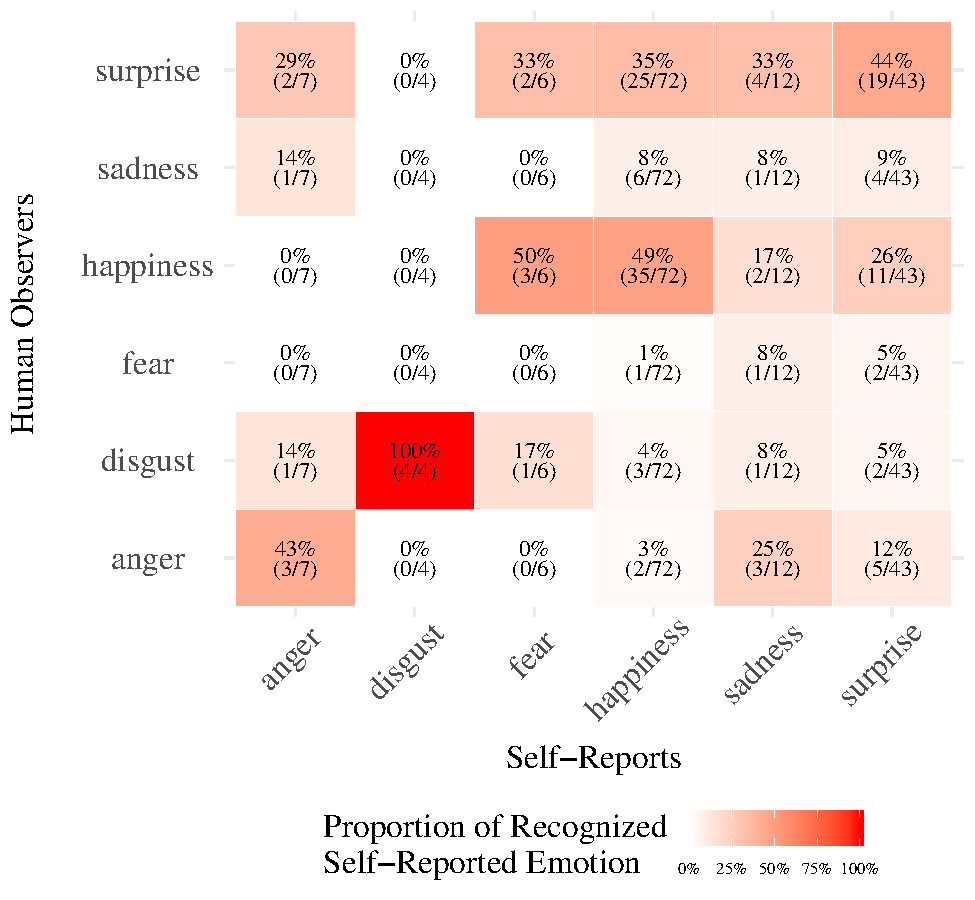
\includegraphics[width=\textwidth]{manuscript_apa_files/figure-latex/confusionMatrix-sr-hr-1} \caption{Confusion matrix between the emotion self-reported as being characteristic of the elicitation with the emotion recognized by the human observers.}\label{fig:confusionMatrix-sr-hr}
\end{figure}

Each emotion label used to describe encoders' self-reported subjective feeling (\emph{i.e.}, the label rated with the highest value) is compared with the emotion labels which were rated with the highest score by human observers. Results of the confusion matrix show a low agreement between the emotion felt by the encoder during the elicitation and the emotion recognized by the human observers (Accuracy = 0.43, 95\% CI {[}0.35,0.52{]}; Kappa = 0.19) except for \emph{disgust} (100\% of the videos self-reported). These results are far from those classically obtained in the literature for emotional facial expression recognition which ranges between 60\% and 80\% accuracy. However these results are mostly obtained with static (\emph{i.e.}, pictures) and posed (\emph{i.e.}, displayed by actors) facial expressions using only 6 emotional labels in a forced-choice paradigm.

Interestingly human observers seem to recognize surprise expressed in videos where anger, fear happiness and sadness was the highest self-reported emotion (respectively 28.6\%, 33.3\%, 34.7\% and 33.3\% of the videos self-reported), and in a lower instance \emph{happiness} was recognized in videos where \emph{fear} and \emph{surprise} was the highest self-reported emotion (respectively 50.0\% and 25.6\% of the videos self-reported).

Sensitivity, specificity, precision and F1 scores for each emotion reveals that \emph{happiness} has the highest coherence ratio whereas \emph{sadness} has the lowest coherence ratio between true positives and false positives (Table \ref{tab:confusionTable-sr-hr}).

\begingroup\fontsize{8}{10}\selectfont

\begin{ThreePartTable}
\begin{TableNotes}[para]
\item Note. *na.* values are produced when not enough data are available to compute accuracy indicators.
\end{TableNotes}
\begin{longtabu} to \linewidth {>{\raggedright}X>{\centering}X>{\centering}X>{\centering}X>{\centering}X}
\caption{\label{tab:confusionTable-sr-hr}Human recognition accuracy metrics for each emotion.}\\
\toprule
Emotion & Sensitivity & Specificity & Precision & F1\\
\midrule
anger & 0.43 & 0.93 & 0.23 & 0.3\\
disgust & 1.00 & 0.94 & 0.33 & 0.5\\
fear & 0.00 & 0.97 & 0.00 & \textit{na.}\\
happiness & 0.49 & 0.78 & 0.69 & 0.57\\
sadness & 0.08 & 0.92 & 0.08 & 0.08\\
surprise & 0.44 & 0.67 & 0.37 & 0.4\\
\bottomrule
\insertTableNotes
\end{longtabu}
\end{ThreePartTable}
\endgroup{}

Accuracy metrics by emotional labels indicate a discrepancy in the ratio of true/false positives. Whereas \emph{happiness} and \emph{disgust} obtain the highest scores, \emph{anger}, \emph{surprise} and \emph{sadness} have the lowest recognition ratio. The underlying effect of expression intensity may explain why \emph{happiness} and \emph{disgust} are easily recognized. \emph{Anger} and \emph{sadness} as non-socially desirable emotions may be have been felt but not expressed.

However, self-reports show a significant proportion of undetermined emotional states (35.2\% of the 358 videos) which reveals the potential limit of using 6-points Likert scales to measure emotional self-reports. Indeed, encoders can easily score to the maximum for more than one emotion.

\hypertarget{automatic-classifiers-accuracy}{%
\subsection{Automatic Classifier's Accuracy}\label{automatic-classifiers-accuracy}}

Similarly to the previous analysis, the overall correlation of recognition and non-recognition revealed a significant but very low coherence between self-reported emotions and automatic classifier's recognition (\(r = .12\), 95\% CI \([.07\), \(.17]\), \(t(1384) = 4.50\), \(p < .001\)). A confusion matrix was used to compare encoders' subjective feeling with the emotion label recognized by the automatic classifier (Figure \ref{fig:confusionMatrix-sr-ar}).

\begin{figure}[!h]
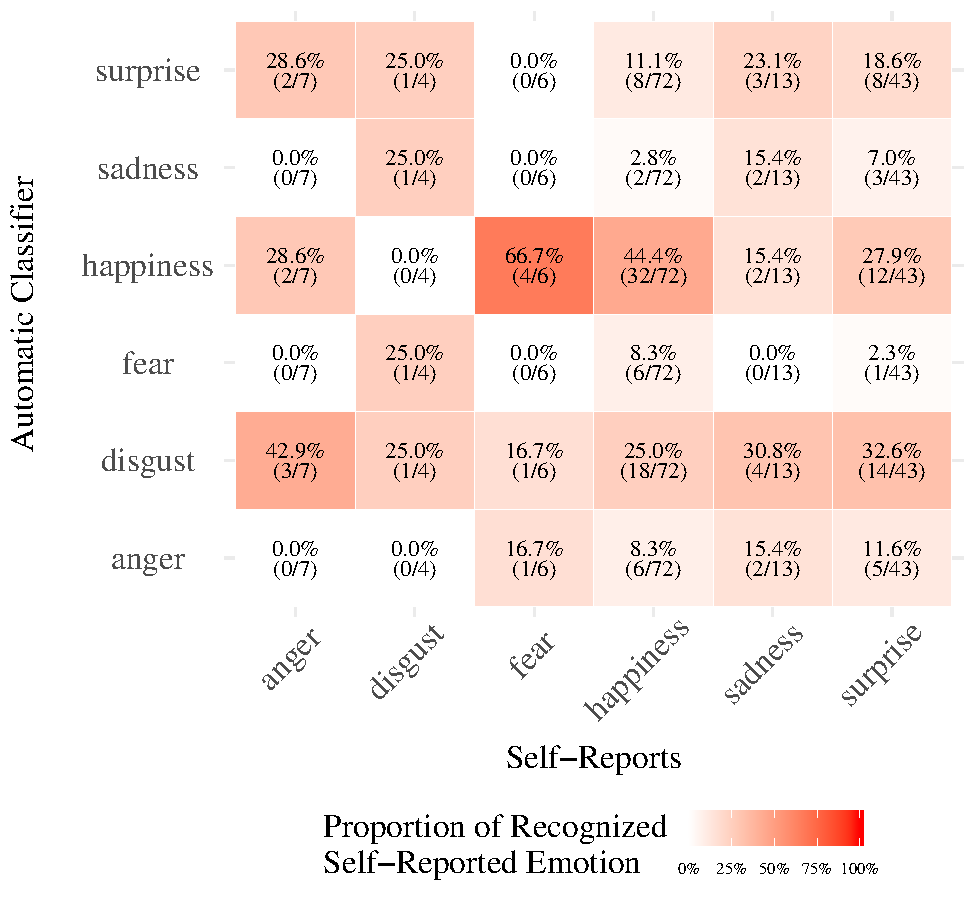
\includegraphics[width=\textwidth]{manuscript_apa_files/figure-latex/confusionMatrix-sr-ar-1} \caption{Confusion matrix of between the emotion self-reported as being characteristic of the elicitation with the emotion recognized by the automatic classifier.}\label{fig:confusionMatrix-sr-ar}
\end{figure}

Results obtained for the comparison between emotions self-reported and recognized by the automatic classifier are somewhat similar to the ones with human observers (Table \ref{tab:confusionTable-sr-ar}). Overall, a low agreement between emotion self-reported and emotion recognized by the automatic classifier (Accuracy = 0.30, 95\% CI {[}0.22,0.38{]}; Kappa = 0.07) except for \emph{happiness} (44.4\% of the video self-reported) is evident.

\begingroup\fontsize{8}{10}\selectfont

\begin{ThreePartTable}
\begin{TableNotes}[para]
\item Note. *na.* values are produced when not enough data are available to compute accuracy indicators.
\end{TableNotes}
\begin{longtabu} to \linewidth {>{\raggedright}X>{\centering}X>{\centering}X>{\centering}X>{\centering}X}
\caption{\label{tab:confusionTable-sr-ar}Autonatic recognition accuracy metrics for each emotion.}\\
\toprule
Emotion & Sensitivity & Specificity & Precision & F1\\
\midrule
anger & 0.00 & 0.90 & 0.00 & \textit{na.}\\
disgust & 0.25 & 0.72 & 0.02 & 0.04\\
fear & 0.00 & 0.94 & 0.00 & \textit{na.}\\
happiness & 0.44 & 0.73 & 0.62 & 0.52\\
sadness & 0.15 & 0.95 & 0.25 & 0.19\\
surprise & 0.19 & 0.86 & 0.36 & 0.25\\
\bottomrule
\insertTableNotes
\end{longtabu}
\end{ThreePartTable}
\endgroup{}

Surprisingly the automatic classifier incorrectly recognized as \emph{disgust} an significant proportion of videos in which \emph{anger}, \emph{happiness} and \emph{surprise} was the highest self-reported emotion (respectively 42.9\%, 25.0\% and 32.6\% of the videos self-reported). In parallel, the automatic classifier recognized as \emph{happiness} videos in which \emph{fear} and \emph{surprise} was the highest self-reported emotion (respectively 66.7\% and 32.6\% of the videos self-reported).

A comparable explanation involving the amount of undetermined video based on self-reports can be provided, as the level of undetermined emotions are very high for the self- reports.

\hypertarget{comparison-between-human-and-automatic-recognition}{%
\subsection{Comparison Between Human and Automatic Recognition}\label{comparison-between-human-and-automatic-recognition}}

As previously mentioned, human observers appear to be more accurate than the automatic classifier to recognize an individual's subjective feeling (human observers Accuracy = 0.43; automatic classifier Accuracy = 0.30; \(r = .22\), 95\% CI \([.17\), \(.27]\), \(t(1384) = 8.31\), \(p < .001\)). However, both make mistakes.

A third confusion matrix is used to compare similarities (diagonal) and differences between human observers and automatic classifier in classifying the six emotion labels (Figure \ref{fig:confusionMatrix-hr-ar}).

\begin{figure}[!h]
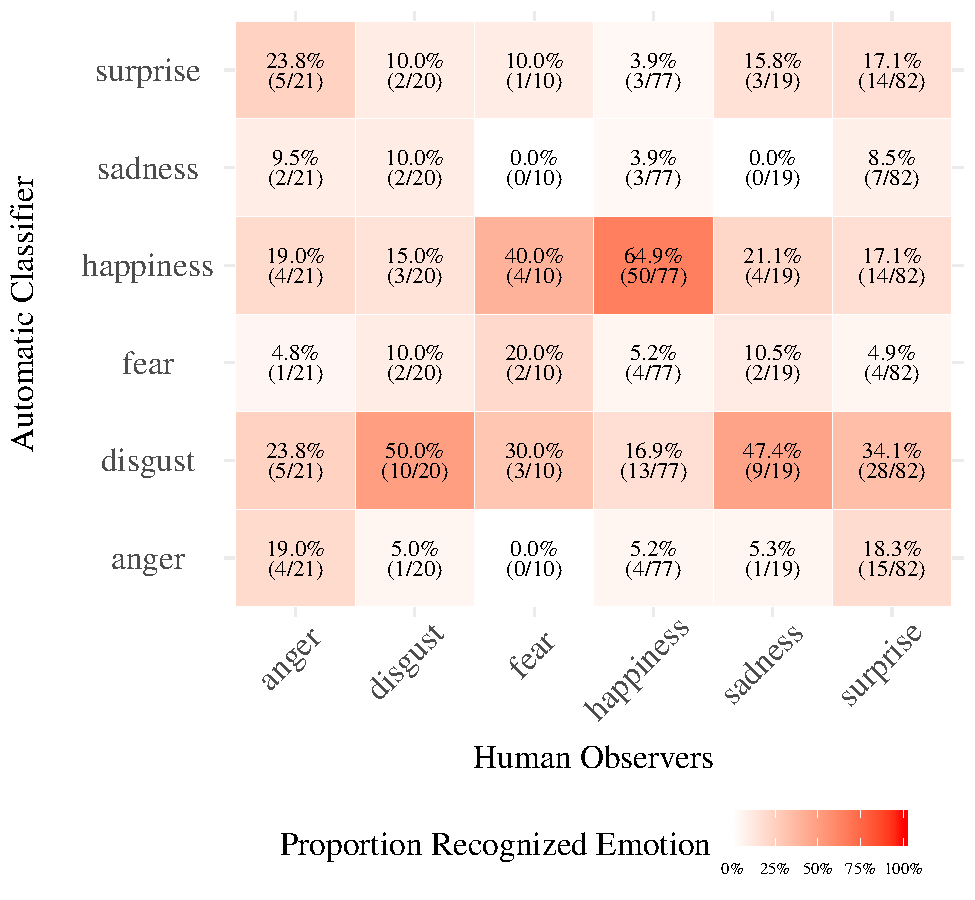
\includegraphics[width=\textwidth]{manuscript_apa_files/figure-latex/confusionMatrix-hr-ar-1} \caption{Proportion of emotion labels classified by human observers which are recognized by the automatif classifier.}\label{fig:confusionMatrix-hr-ar}
\end{figure}

The overall agreement between human observers and the automatic classifier is in fact very low (Kappa = 0.18). Except for \emph{happiness} and \emph{disgust} (respectively 64.9\% and 50.0\% of common labelling), there is no clear common pattern. Moreover, the automatic classifier has a tendency to label as \emph{disgust} videos labeled as \emph{sadness} by human observers, and as \emph{happiness} videos labeled as \emph{fear} by human observers.

\hypertarget{discussion-and-conclusion}{%
\subsection{Discussion and Conclusion}\label{discussion-and-conclusion}}

Despite being one of the most investigated questions in affective science, the consistency between emotion felt and facially displayed on the one hand, and facial expression recognized on the other is a hot topic. To date no clear evidence has been found to definitively solve the questions raised. Yet, with the growing interest of industries and government in monitoring individual's psychological states, this issue is under intense scrutiny. The present research aims to provide some empirical data to answer some of the questions posed. The faces encoders spontaneously displayed when confronted with an emotional eliciting task were submitted both to human and to automatic recognition. The criterion for recognition accuracy was the subjective feeling self-reported by the encoder once the elicitation task was carried out. Results first reveal a low consistency between emotion felt and facial expression displayed. They show that facial expressions of emotion are often not displayed when the Basic Emotion View would predict them to be expressed. Secondly, results show low accuracy rates for both humans and the automatic classifier in identifying the inner emotional states of these encoders based on their facial expressions. Thirdly, human observers prove to be better at recognizing the emotion facially expressed than the automatic recognition tool is. Such results support the hypothesis advanced by some authors of low emotion--expression coherence (Kappas, 2003). In many instances, facial displays are not associated with a concordant emotional state, even any emotional state at all (Bonanno \& Keltner, 2004; Fernández-Dols \& Crivelli, 2013). More and more evidence is showing that facial expressions are in reality not expressing emotions (McKeown, 2013). Increasing studies show that, for most emotions, the EFE elicited by emotional triggers are scarce and partial, even when micro-expressions are taken into account (Durán et al., 2017). These studies are conducted either in laboratory settings or in the field. This is not to say that facial expression is not an informative modality for understanding the emotional state of a person. There is indeed an affinity between emotion and facial display (Frijda \& Tcherkassof, 1997). However, claiming that there are unique \enquote{signatures} allowing using configurations of facial muscles to infer the presence of a specific emotion is misleading. As well as other nonverbal behaviors, facial movements are not only assumed to be determined by emotion but also by various other causes, such as psychological states (\emph{e.g.}, motivations or pain), to say nothing of social context and sociocultural norms (Ekman et al., 1987). Hence, facial movements have causes and functions other than the expression of emotion. This multiple determination excludes any possibility of drawing a linear inference from facial activity on the underlying psychological state (emotional or other). Beyond the present observations showing a weak consistency between subjective feelings and spontaneous facial expressions, this study sheds some light on the controversy between the Basic Emotion View and the constructivist approach as to the facial recognition issue. The former (Ekman, 1992) assumes that expressions of emotion are brief and coherent patterns of facial muscle movements that co-vary with discrete subjective experiences. In return, this information displayed by the face corresponds to the one extracted by perceivers. Instead of viewing emotions as natural kinds (Barrett, 2006), the constructivist approach supposes that emotions are social constructions and that facial behaviors intrinsically situated. The emotions that are recognized by the observer are constructed in her/his mind. Therefore, facial movements do not express specific emotions because they do not carry intrinsic emotional signification. It is the observer that infers the emotional meaning of the facial expression, this interpretation depending on availability of different information such as context or linguistic categories. As a consequence, one can predict from the first line of thinking that individuals' emotional subjective feeling should be correlated to the recognition of facial expressions from both human observers and automatic classifiers whereas if emotions are social constructs, as stated by the second line of thinking, human observer's should be better at perceiving emotions expressed on the face than automatic classifiers.

The present findings speak against any strong version of the Basic Emotion View. The correlations between the self-measured emotions and the observed facial behaviors are low and the latter are weakly recognized. Present results plead instead in favor of the constructivist stance. They show that human observers are more accurate than the automatic recognition tool to identify an individual's subjective feeling on the basis of their face. Moreover, mistakes made by human observers look less arbitrary to the ones made by the classifier. For instance, even if a mix-up between disgust and anger is sometimes reported in recognition studies, odd confusions such as the present ones produced by the classifier have never been noted for human observers. The latter obviously make sense of the facial behavior they are witnessing. However, the human decoders in the present study were presented with faces without any contextual information which could have helped them to shape more precisely their interpretation. Hassin, Aviezer, \& Bentin (2013) reviewed evidence to demonstrate that faces are inherently ambiguous and that observers rely on situational cues when they process facial displays (see also Aviezer et al., 2008; Barrett, Mesquita, \& Gendron, 2011). It happens that contextual information even shifts emotion perception. In the present case, the facial stimuli displayed to the decoders were as equivocal as are real-life facial expressions (Aviezer, Ensenberg, \& Hassin, 2017). Yet, decoders had no cue at disposal. So, without any possibility of integrating faces and context, their decoding accuracy is pretty much degraded as it is usual in such cases (\emph{e.g.}, Wagner, MacDonald, \& Manstead, 1986). However, they demonstrate their superiority on the classifier tool probably thanks to their capacity to rely on their previous personal experience to invent a context in which a face could display such an expression. Once a credible context retrieved, they can affix an emotional label to the facial behavior.

Several limitations should be stated, highlighting the need for further research. One of them is effectiveness of the emotion elicitation tasks. One can consider that an intensity threshold needs to be exceeded for a visible emotional expression to occur. In the case of the present study, it may be that insufficient emotion intensity accounts for the low number of visibly reactive participants. However, such line of reasoning fits badly with the Basic Emotion View according to which emotions and their related prototypical facial behavior are universal because they are considered as innate mechanisms allowing individuals to respond adaptively to evolutionary significant events (threats, opportunities\ldots{}) encountered in the environment, whatever their potency. Moreover, various studies have used fairly strong emotion inductions without obtaining any visible facial display of any kind of emotion (Durán et al., 2017). Besides, the present results show a quite good correlation between reported emotion and facial behavior for happiness. Thus, there are no reasons to believe that an explanation in terms of a too low emotion threshold applies for the other emotions under consideration. The latter were triggered and measured with conceptually identical elicitation and assessment procedures (Reisenzein et al., 2013). The use of self-reports to evaluate encoders' subjective feelings is another limitation that can also be put forward because of the numerous cognitive biases they entail. Well known problems with the reliability of self-reports are, among others, the reconstructive nature of memory, the influence of attentional biases on reports, demand characteristics, distorting effects of implicit causal theories and personal motives, as stressed by Nielsen \& Kaszniak (2007). It is clearly obvious that self-reports are not simple outlets of inner mental processes but personal constructions and they are affected by many factors (Kappas, 2003). The emotional feeling echoes motivational tendencies, bodily changes, and cognitive appraisals of events (Sander \& Scherer, 2014). All these are encapsulated into semantic categories referred to by labels. As things stand currently, there is unfortunately no objective way for accessing and assessing inner subjective emotional feelings except for asking people to report their subjective experience in words. The procedure used for human recognition can also be open to dispute. First, one can criticize the decoders' expertise level since they were not FACS coders but untrained students. Of course one can expect a difference between skilled annotators and novice ones regarding the assessment of emotional facial displays. This said, in everyday life, few people are specialist coders yet the quantity of successful social interactions proves lay persons recognize pretty well others' facial behaviors. Therefore, and especially in the interest of generalizability, asking inexpert people seems relevant. Secondly, instead of using a classic forced-choice procedure, a more subtle approach was chosen to mimic results provided by the automatic classifier. As explained above, annotators first delimitated a temporal sequence during which they noticed an emotional display on the face, and then attributed an emotion label to this behavioral sequence in a second step. Whereas this paradigm is longer and more complicated, it can lead to more robust results in reducing the forced-choice bias (Russell, 1993). However this procedure can also reduce the human observers' accuracy. In this regard, the results of the human observation could have been more ambiguous because it is not the natural way that people are inferring meaning from facial expressions. An alternative explanation relies in reducing the recognition bias involved in the classic recognition paradigm. Classic forced-choice paradigms obtain artificially high results, thus by using a more evolved approach observers' accuracy may have been lowered. Another flaw is the lack of comparison with various facial expression recognition methods. Human recognition has only been compared to the Affdex classifier. Future studies are needed to confront human assessments with different automatic recognition methods, both frame based methods and sequence based automatic ones. This latter issue is particularly decisive. Indeed, the issue of the recognition of dynamic expressive sequences is essential because ordinary facial behavior is made up of dynamically shifting morphological features (Krumhuber, Kappas, \& Manstead, 2013). This temporal information is indisputably a key feature of facial activity. Not only observer-based judgements of facial displays must be compared to automated facial analysis, but also different kinds of human recognition measurements should be undertaken. The challenge researchers are especially confronted with is to find ways to appropriately collect data regarding the perception of spontaneous and dynamic facial behavior. Finally, our understanding of facial displays as they occur in everyday interactions requires a strong emphasis on ecological concerns. The present study is a laboratory experiment. It has the advantage of controlling different parameters of the emotions investigated, such as intensity, quality, and temporal (onset, duration) features. Moreover, as encoders are alone, facing an emotional trigger, it also controls for the social context, removing its possible influence on their facial behaviors. However, it is known that encoders' imagination can influence their expressiveness, for instance when they believe that their friend is doing the same (\emph{vs.} a different) emotional task in another room (Jakobs, Manstead, \& Fischer, 1999). Trying to exclude social influence by leaving encoders alone may be illusionary then. From an ecological perspective, it is even a mistake to exonerate behavioral observations from social contexts. Facial activity measurement in dyadic interactions has shown that the facial behavior of the perceiver reflects sometimes more what the expresser is experiencing than what the perceiver is feeling. It is the case, for instance, of emotional mimicry in dynamic social interactions (Hess \& Fischer, 2016). It is also the case of healthy partners interacting with schizophrenic patients whose facial activity is pretty much identical (Krause, Steimer-Krause, Merten, \& Ullrich, 1998). Hence, in order to better comprehend emotional communication in human relationships, experimental research should be corroborated with more ecological protocols.

Nowadays, automatic recognition systems are based on the coding of the facial muscular activations from which they infer the expressed emotion. Such automatic classifier tools take for granted that, when experienced, firstly an emotion is displayed on the face, secondly, in the form of a configuration of facial muscles that is all his own, and thirdly, which is recognized by the perceiver (be it a human being or an automatic system). These are the Basic Emotion View assertions, jeopardized by field observations and laboratory experiments on spontaneous expression of emotions, such as the present study. All raise serious objections to the supposed close relation between emotion and face. They bring up several questions regarding the role the context plays in the emission and interpretation of the so-called facial expression of emotion. The finalization of operational and effective \enquote{reading emotional faces} devices rests on their answer. As a result, despite being one of the most investigated questions in affective science, the growing interest of industries and governments in tracking individual's psychological states is hardly given satisfaction. Considering the above, the present results provide additional evidence that an individual's subjective feeling cannot be inferred from facial expressions and in our case invalidate the hypothesis of hardwired emotions unambiguously displayed on the face. Even if emotions were hardwired, in everyday life one does not observe prototypical facial expressions because of their rarity and therefore research should be focused on analyzing non-prototypical facial expressions. Advancements in identifying \enquote{non-basic} emotion labels as well as non-prototypical facial expression have indeed been made in the development of automatic facial expression recognition tools (McDuff, 2016). However, these present results suggest that automatic facial expression recognition tools should merely evaluate facial morphology features such as action units (already evaluated in OpenFace, Baltrušaitis, Robinson, \& Morency, 2016, Affectiva's Affdex, McDuff et al. (2016), or Vicar Vision's FaceReader, Den Uyl and Van Kuilenburg (2005), to name a few) rather than inferring supposedly emotional or affective states. Trying to interpret facial displays as a means of determining underlying emotional state, in all likelihood, remains vain.

\newpage

\hypertarget{references}{%
\section{References}\label{references}}

\begingroup
\setlength{\parindent}{-0.5in}
\setlength{\leftskip}{0.5in}

\hypertarget{refs}{}
\leavevmode\hypertarget{ref-aviezer2017inherently}{}%
Aviezer, H., Ensenberg, N., \& Hassin, R. R. (2017). The inherently contextualized nature of facial emotion perception. \emph{Current Opinion in Psychology}, \emph{17}, 47--54.

\leavevmode\hypertarget{ref-aviezer2008angry}{}%
Aviezer, H., Hassin, R. R., Ryan, J., Grady, C., Susskind, J., Anderson, A., \ldots{} Bentin, S. (2008). Angry, disgusted, or afraid? Studies on the malleability of emotion perception. \emph{Psychological Science}, \emph{19}(7), 724--732.

\leavevmode\hypertarget{ref-baltruvsaitis2016openface}{}%
Baltrušaitis, T., Robinson, P., \& Morency, L.-P. (2016). Openface: An open source facial behavior analysis toolkit. In \emph{2016 ieee winter conference on applications of computer vision (wacv)} (pp. 1--10). IEEE.

\leavevmode\hypertarget{ref-barrett2006emotions}{}%
Barrett, L. F. (2006). Are emotions natural kinds? \emph{Perspectives on Psychological Science}, \emph{1}(1), 28--58.

\leavevmode\hypertarget{ref-barrett2019emotional}{}%
Barrett, L. F., Adolphs, R., Marsella, S., Martinez, A. M., \& Pollak, S. D. (2019). Emotional expressions reconsidered: Challenges to inferring emotion from human facial movements. \emph{Psychological Science in the Public Interest}, \emph{20}(1), 1--68.

\leavevmode\hypertarget{ref-barrett2011context}{}%
Barrett, L. F., Mesquita, B., \& Gendron, M. (2011). Context in emotion perception. \emph{Current Directions in Psychological Science}, \emph{20}(5), 286--290.

\leavevmode\hypertarget{ref-bennett2002facial}{}%
Bennett, D. S., Bendersky, M., \& Lewis, M. (2002). Facial expressivity at 4 months: A context by expression analysis. \emph{Infancy}, \emph{3}(1), 97--113.

\leavevmode\hypertarget{ref-bonanno2004brief}{}%
Bonanno, G., \& Keltner, D. (2004). The coherence of emotion systems: Comparing ``on-line'' measures of appraisal and facial expressions, and self-report. \emph{Cognition and Emotion}, \emph{18}(3), 431--444. \url{https://doi.org/10.1080/02699930341000149}

\leavevmode\hypertarget{ref-buck1985prime}{}%
Buck, R. (1985). Prime theory: An integrated view of motivation and emotion. \emph{Psychological Review}, \emph{92}(3), 389.

\leavevmode\hypertarget{ref-camras1991development}{}%
Camras, L. A., Malatesta, C., \& Izard, C. E. (1991). The development of facial expressions in infancy.

\leavevmode\hypertarget{ref-camras2007infants}{}%
Camras, L. A., Oster, H., Bakeman, R., Meng, Z., Ujiie, T., \& Campos, J. J. (2007). Do infants show distinct negative facial expressions for fear and anger? Emotional expression in 11-month-old european american, chinese, and japanese infants. \emph{Infancy}, \emph{11}(2), 131--155.

\leavevmode\hypertarget{ref-cohn2003timing}{}%
Cohn, J. F., \& Schmidt, K. (2003). The timing of facial motion in posed and spontaneous smiles. In \emph{Active media technology} (pp. 57--69). World Scientific.

\leavevmode\hypertarget{ref-crivelli2015smiles}{}%
Crivelli, C., Carrera, P., \& Fernández-Dols, J.-M. (2015). Are smiles a sign of happiness? Spontaneous expressions of judo winners. \emph{Evolution and Human Behavior}, \emph{36}(1), 52--58.

\leavevmode\hypertarget{ref-crivelli2018facial}{}%
Crivelli, C., \& Fridlund, A. J. (2018). Facial displays are tools for social influence. \emph{Trends in Cognitive Sciences}, \emph{22}(5), 388--399. \url{https://doi.org/10.1016/j.tics.2018.02.006}

\leavevmode\hypertarget{ref-crivelli2017recognizing}{}%
Crivelli, C., Russell, J. A., Jarillo, S., \& Fernández-Dols, J.-M. (2017). Recognizing spontaneous facial expressions of emotion in a small-scale society of papua new guinea. \emph{Emotion}, \emph{17}(2), 337.

\leavevmode\hypertarget{ref-darwin1872expression}{}%
Darwin, C. (1872). \emph{The expression of the emotions in man and animals}. London, UK: John Murray.

\leavevmode\hypertarget{ref-dente2017measures}{}%
Dente, P., Küster, D., Skora, L., \& Krumhuber, E. (2017). Measures and metrics for automatic emotion classification via facet. In \emph{Proceedings of the conference on the study of artificial intelligence and simulation of behaviour} (pp. 160--163).

\leavevmode\hypertarget{ref-den2005facereader}{}%
Den Uyl, M., \& Van Kuilenburg, H. (2005). The facereader: Online facial expression recognition. In \emph{Proceedings of measuring behavior} (Vol. 30, pp. 589--590). Citeseer.

\leavevmode\hypertarget{ref-digirolamo2017emotion}{}%
DiGirolamo, M. A., \& Russell, J. A. (2017). The emotion seen in a face can be a methodological artifact: The process of elimination hypothesis. \emph{Emotion}, \emph{17}(3), 538.

\leavevmode\hypertarget{ref-dols2017natural}{}%
Dols, J. M. F. (2017). Natural facial expression: A view from psychological constructionism and pragmatics. In J. M. F. Dols \& J. A. Russell (Eds.), \emph{The science of facial expression} (pp. 457--478). New York, NY: Oxford University Press.

\leavevmode\hypertarget{ref-duchenne1876mecanisme}{}%
Duchenne, G.-B. (1876). \emph{Mécanisme de la physionomie humaine: Où, analyse électro-physiologique de l'expression des passions}. J.-B. Baillière.

\leavevmode\hypertarget{ref-dupre2015oudjat}{}%
Dupré, D., Akpan, D., Elias, E., Adam, J.-M., Meillon, B., Bonnefond, N., \ldots{} Tcherkassof, A. (2015). Oudjat: A configurable and usable annotation tool for the study of facial expressions of emotion. \emph{International Journal of Human-Computer Studies}, \emph{83}, 51--61. \url{https://doi.org/10.1016/j.ijhcs.2015.05.010}

\leavevmode\hypertarget{ref-dupre2018accuracy}{}%
Dupré, D., Andelic, N., Morrison, G., \& McKeown, G. (2018). Accuracy of three commercial automatic emotion recognition systems across different individuals and their facial expressions. In \emph{Proceedings of the international conference on pervasive computing and communications} (pp. 627--632). \url{https://doi.org/10.1109/PERCOMW.2018.8480127}

\leavevmode\hypertarget{ref-duran2017coherence}{}%
Durán, J. I., Reisenzein, R., \& Fernández-Dols, J.-M. (2017). Coherence between emotions and facial expressions, 107--129.

\leavevmode\hypertarget{ref-ekman1992argument}{}%
Ekman, P. (1992). An argument for basic emotions. \emph{Cognition \& Emotion}, \emph{6}(3-4), 169--200. \url{https://doi.org/10.1080/02699939208411068}

\leavevmode\hypertarget{ref-ekman2007directed}{}%
Ekman, P. (2007). The directed facial action task. In J. A. Coan \& J. J. B. Allen (Eds.), \emph{Handbook of emotion elicitation and assessment} (pp. 47--53). New York, NY: Oxford University Press.

\leavevmode\hypertarget{ref-ekman2017facial}{}%
Ekman, P. (2017). Facial expressions. In J.-M. Fernández-Dols \& J. A. Russell (Eds.), \emph{The science of facial expression} (pp. 39--56). New York, NY: Oxford University Press.

\leavevmode\hypertarget{ref-ekman2011meant}{}%
Ekman, P., \& Cordaro, D. (2011). What is meant by calling emotions basic. \emph{Emotion Review}, \emph{3}(4), 364--370.

\leavevmode\hypertarget{ref-ekman1980facial}{}%
Ekman, P., Freisen, W. V., \& Ancoli, S. (1980). Facial signs of emotional experience. \emph{Journal of Personality and Social Psychology}, \emph{39}(6), 1125.

\leavevmode\hypertarget{ref-ekman1987universals}{}%
Ekman, P., Friesen, W. V., O'sullivan, M., Chan, A., Diacoyanni-Tarlatzis, I., Heider, K., \ldots{} Tomita, M. (1987). Universals and cultural differences in the judgments of facial expressions of emotion. \emph{Journal of Personality and Social Psychology}, \emph{53}(4), 712--717. \url{https://doi.org/10.1037/0022-3514.53.4.712}

\leavevmode\hypertarget{ref-ekman1988universality}{}%
Ekman, P., \& Heider, K. G. (1988). The universality of a contempt expression: A replication. \emph{Motivation and Emotion}, \emph{12}(3), 303--308. \url{https://doi.org/10.1007/BF00993116}

\leavevmode\hypertarget{ref-elfenbein2002universality}{}%
Elfenbein, H. A., \& Ambady, N. (2002). On the universality and cultural specificity of emotion recognition: A meta-analysis. \emph{Psychological Bulletin}, \emph{128}(2), 203.

\leavevmode\hypertarget{ref-fernandez1997spontaneous}{}%
Fernandez-Dols, J.-M., Sanchez, F., Carrera, P., \& Ruiz-Belda, M.-A. (1997). Are spontaneous expressions and emotions linked? An experimental test of coherence. \emph{Journal of Nonverbal Behavior}, \emph{21}(3), 163--177.

\leavevmode\hypertarget{ref-fernandez2013emotion}{}%
Fernández-Dols, J.-M., \& Crivelli, C. (2013). Emotion and expression: Naturalistic studies. \emph{Emotion Review}, \emph{5}(1), 24--29. \url{https://doi.org/10.1177/1754073912457229}

\leavevmode\hypertarget{ref-fernandez1995smiles}{}%
Fernández-Dols, J.-M., \& Ruiz-Belda, M.-A. (1995). Are smiles a sign of happiness? Gold medal winners at the olympic games. \emph{Journal of Personality and Social Psychology}, \emph{69}(6), 1113.

\leavevmode\hypertarget{ref-fridlund1994human}{}%
Fridlund, A. J. (1994). \emph{Human facial expression: An evolutionary view}. San Diego, CA: Academic Press.

\leavevmode\hypertarget{ref-frijda2012recognition}{}%
Frijda, N. (2012). Recognition of emotion in others. In F. Paglieri (Ed.), \emph{Consciousness in interaction. The role of the natural and social context in shaping consciousness} (pp. 237--256). Amsterdam, NL: J.Benjamins.

\leavevmode\hypertarget{ref-frijda1997facial}{}%
Frijda, N. H., \& Tcherkassof, A. (1997). Facial expressions as modes of action readiness. In J. A. Russell \& J.-M. Fernández-Dols (Eds.), \emph{The psychology of facial expression} (pp. 78--102). New York, NY: Cambridge University Press.

\leavevmode\hypertarget{ref-gendron2018emotion}{}%
Gendron, M., Hoemann, K., Crittenden, A. N., Msafiri, S., Ruark, G. A., \& Barrett, L. F. (2018). Emotion perception in hadza hunter gatherers.

\leavevmode\hypertarget{ref-gendron2014perceptions}{}%
Gendron, M., Roberson, D., Vyver, J. M. van der, \& Barrett, L. F. (2014). Perceptions of emotion from facial expressions are not culturally universal: Evidence from a remote culture. \emph{Emotion}, \emph{14}(2), 251.

\leavevmode\hypertarget{ref-hassin2013inherently}{}%
Hassin, R. R., Aviezer, H., \& Bentin, S. (2013). Inherently ambiguous: Facial expressions of emotions, in context. \emph{Emotion Review}, \emph{5}(1), 60--65.

\leavevmode\hypertarget{ref-hess2016emotional}{}%
Hess, U., \& Fischer, A. H. (2016). \emph{Emotional mimicry in social context}. Cambridge University Press.

\leavevmode\hypertarget{ref-hess1990differentiating}{}%
Hess, U., \& Kleck, R. E. (1990). Differentiating emotion elicited and deliberate emotional facial expressions. \emph{European Journal of Social Psychology}, \emph{20}(5), 369--385.

\leavevmode\hypertarget{ref-jakobs1999social}{}%
Jakobs, E., Manstead, A. S., \& Fischer, A. H. (1999). Social motives and emotional feelings as determinants of facial displays: The case of smiling. \emph{Personality and Social Psychology Bulletin}, \emph{25}(4), 424--435.

\leavevmode\hypertarget{ref-johnson2010smile}{}%
Johnson, K. J., Waugh, C. E., \& Fredrickson, B. L. (2010). Smile to see the forest: Facially expressed positive emotions broaden cognition. \emph{Cognition and Emotion}, \emph{24}(2), 299--321.

\leavevmode\hypertarget{ref-kamachi2013dynamic}{}%
Kamachi, M., Bruce, V., Mukaida, S., Gyoba, J., Yoshikawa, S., \& Akamatsu, S. (2013). Dynamic properties influence the perception of facial expressions. \emph{Perception}, \emph{42}(11), 1266--1278.

\leavevmode\hypertarget{ref-kanade2000comprehensive}{}%
Kanade, T., Cohn, J. F., \& Tian, Y. (2000). Comprehensive database for facial expression analysis. In \emph{Proceedings fourth ieee international conference on automatic face and gesture recognition (cat. No. PR00580)} (pp. 46--53). IEEE.

\leavevmode\hypertarget{ref-kappas2003facial}{}%
Kappas, A. (2003). What facial activity can and cannot tell us about emotions. In M. Katsikitis (Ed.), \emph{The human face} (pp. 215--234). Boston, MA: Springer.

\leavevmode\hypertarget{ref-krause1998dyadic}{}%
Krause, R., Steimer-Krause, E., Merten, J., \& Ullrich, B. (1998). Dyadic interaction regulation, emotion, and psychopathology. \emph{Emotions and Psychopathology: Theory and Research}, 70--80.

\leavevmode\hypertarget{ref-kraut1979social}{}%
Kraut, R. E., \& Johnston, R. E. (1979). Social and emotional messages of smiling: An ethological approach. \emph{Journal of Personality and Social Psychology}, \emph{37}(9), 1539--1553.

\leavevmode\hypertarget{ref-krumhuber2013effects}{}%
Krumhuber, E. G., Kappas, A., \& Manstead, A. S. (2013). Effects of dynamic aspects of facial expressions: A review. \emph{Emotion Review}, \emph{5}(1), 41--46.

\leavevmode\hypertarget{ref-lee2002effect}{}%
Lee, V., \& Wagner, H. (2002). The effect of social presence on the facial and verbal expression of emotion and the interrelationships among emotion components. \emph{Journal of Nonverbal Behavior}, \emph{26}(1), 3--25.

\leavevmode\hypertarget{ref-lindquist2006language}{}%
Lindquist, K. A., Barrett, L. F., Bliss-Moreau, E., \& Russell, J. A. (2006). Language and the perception of emotion. \emph{Emotion}, \emph{6}(1), 125.

\leavevmode\hypertarget{ref-lindquist2013s}{}%
Lindquist, K. A., \& Gendron, M. (2013). What's in a word? Language constructs emotion perception. \emph{Emotion Review}, \emph{5}(1), 66--71. \url{https://doi.org/10.1177/1754073912451351}

\leavevmode\hypertarget{ref-mcduff2016discovering}{}%
McDuff, D. (2016). Discovering facial expressions for states of amused, persuaded, informed, sentimental and inspired. In \emph{Proceedings of the international conference on multimodal interaction} (pp. 71--75). \url{https://doi.org/10.1145/2993148.2993192}

\leavevmode\hypertarget{ref-mcduff2016affdex}{}%
McDuff, D., Mahmoud, A., Mavadati, M., Amr, M., Turcot, J., \& Kaliouby, R. el. (2016). AFFDEX sdk: A cross-platform real-time multi-face expression recognition toolkit. In \emph{Proceedings of the chi conference on human factors in computing systems} (pp. 3723--3726). \url{https://doi.org/10.1145/2851581.2890247}

\leavevmode\hypertarget{ref-mckeown2013analogical}{}%
McKeown, G. J. (2013). The analogical peacock hypothesis: The sexual selection of mind-reading and relational cognition in human communication. \emph{Review of General Psychology}, \emph{17}(3), 267--287. \url{https://doi.org/10.1037/a0032631}

\leavevmode\hypertarget{ref-mehu2007smiles}{}%
Mehu, M., Grammer, K., \& Dunbar, R. I. (2007). Smiles when sharing. \emph{Evolution and Human Behavior}, \emph{28}(6), 415--422.

\leavevmode\hypertarget{ref-meillon2010dynemo}{}%
Meillon, B., Tcherkassof, A., Mandran, N., Adam, J.-M., Dubois, M., Dupré, D., \ldots{} Caplier, A. (2010). DynEmo: A corpus of dynamic and spontaneous emotional facial expressions. In \emph{Proceedings of international workshop series on multimodal corpora, tools and resources. Multimodal corpora: Advances in capturing, coding and analyzing multimodality} (pp. 31--36).

\leavevmode\hypertarget{ref-nielsen2007conceptual}{}%
Nielsen, L., \& Kaszniak, A. W. (2007). Conceptual, theoretical, and methodological issues in inferring subjective emotion experience. \emph{Handbook of Emotion Elicitation and Assessment}, 361--375.

\leavevmode\hypertarget{ref-pacherie2003modes}{}%
Pacherie, E. (2003). Modes de structuration des contenus perceptifs visuels. \emph{J. Bouveresse \& J.-J. Rosat (Eds), Philosophies de La Perception. Phénoménologie, Grammaire et Sciences Cognitives, Paris: Odile Jacob}, 263--289.

\leavevmode\hypertarget{ref-reisenzein2000exploring}{}%
Reisenzein, R. (2000). Exploring the strength of association between the components of emotion syndromes: The case of surprise. \emph{Cognition \& Emotion}, \emph{14}(1), 1--38.

\leavevmode\hypertarget{ref-reisenzein2006evidence}{}%
Reisenzein, R., Bördgen, S., Holtbernd, T., \& Matz, D. (2006). Evidence for strong dissociation between emotion and facial displays: The case of surprise. \emph{Journal of Personality and Social Psychology}, \emph{91}(2), 295.

\leavevmode\hypertarget{ref-reisenzein2013coherence}{}%
Reisenzein, R., Studtmann, M., \& Horstmann, G. (2013). Coherence between emotion and facial expression: Evidence from laboratory experiments. \emph{Emotion Review}, \emph{5}(1), 16--23.

\leavevmode\hypertarget{ref-rosenberg1994coherence}{}%
Rosenberg, E. L., \& Ekman, P. (1994). Coherence between expressive and experiential systems in emotion. \emph{Cognition \& Emotion}, \emph{8}(3), 201--229.

\leavevmode\hypertarget{ref-ruiz2003spontaneous}{}%
Ruiz-Belda, M.-A., Fernández-Dols, J.-M., Carrera, P., \& Barchard, K. (2003). Spontaneous facial expressions of happy bowlers and soccer fans. \emph{Cognition and Emotion}, \emph{17}(2), 315--326.

\leavevmode\hypertarget{ref-russell1993forced}{}%
Russell, J. A. (1993). Forced-choice response format in the study of facial expression. \emph{Motivation and Emotion}, \emph{17}(1), 41--51. \url{https://doi.org/10.1007/BF00995206}

\leavevmode\hypertarget{ref-russell1994there}{}%
Russell, J. A. (1994). Is there universal recognition of emotion from facial expression? A review of the cross-cultural studies. \emph{Psychological Bulletin}, \emph{115}(1), 102.

\leavevmode\hypertarget{ref-russell2003facial}{}%
Russell, J. A., Bachorowski, J.-A., \& Fernández-Dols, J.-M. (2003). Facial and vocal expressions of emotion. \emph{Annual Review of Psychology}, \emph{54}(1), 329--349.

\leavevmode\hypertarget{ref-russell1987relativity}{}%
Russell, J. A., \& Fehr, B. (1987). Relativity in the perception of emotion in facial expressions. \emph{Journal of Experimental Psychology: General}, \emph{116}(3), 223.

\leavevmode\hypertarget{ref-sander2014oxford}{}%
Sander, D., \& Scherer, K. (2014). \emph{Oxford companion to emotion and the affective sciences}. OUP Oxford.

\leavevmode\hypertarget{ref-scherer1997lost}{}%
Scherer, K. R., \& Ceschi, G. (1997). Lost luggage: A field study of emotion--antecedent appraisal. \emph{Motivation and Emotion}, \emph{21}(3), 211--235.

\leavevmode\hypertarget{ref-schutzwohl2012facial}{}%
Schützwohl, A., \& Reisenzein, R. (2012). Facial expressions in response to a highly surprising event exceeding the field of vision: A test of darwin's theory of surprise. \emph{Evolution and Human Behavior}, \emph{33}(6), 657--664.

\leavevmode\hypertarget{ref-tcherkassof2007facial}{}%
Tcherkassof, A., Bollon, T., Dubois, M., Pansu, P., \& Adam, J.-M. (2007). Facial expressions of emotions: A methodological contribution to the study of spontaneous and dynamic emotional faces. \emph{European Journal of Social Psychology}, \emph{37}(6), 1325--1345.

\leavevmode\hypertarget{ref-tcherkassof2013dynemo}{}%
Tcherkassof, A., Dupré, D., Meillon, B., Mandran, N., Dubois, M., \& Adam, J.-M. (2013). DynEmo: A video database of natural facial expressions of emotions. \emph{The International Journal of Multimedia \& Its Applications}, \emph{5}(5), 61--80. \url{https://doi.org/10.5121/ijma.2013.5505}

\leavevmode\hypertarget{ref-tcherkassof2014emotions}{}%
Tcherkassof, A., \& Frijda, N. H. (2014). Les émotions: Une conception relationnelle. \emph{LAnnee Psychologique}, \emph{114}(3), 501--535.

\leavevmode\hypertarget{ref-tsai2002emotional}{}%
Tsai, J. L., Chentsova-Dutton, Y., Freire-Bebeau, L., \& Przymus, D. E. (2002). Emotional expression and physiology in european americans and hmong americans. \emph{Emotion}, \emph{2}(4), 380.

\leavevmode\hypertarget{ref-vernon2002disgust}{}%
Vernon, L. L., \& Berenbaum, H. (2002). Disgust and fear in response to spiders. \emph{Cognition \& Emotion}, \emph{16}(6), 809--830.

\leavevmode\hypertarget{ref-de2019mama}{}%
Waal, F. de. (2019). \emph{Mama's last hug: Animal emotions and what they teach us about ourselves}. London, UK: Granta Books.

\leavevmode\hypertarget{ref-wagner1997methods}{}%
Wagner, H. L. (1997). Methods for the study of facial behavior. In J. A. Russell \& J.-M. Fernández-Dols (Eds.), \emph{The psychology of facial expression} (pp. 31--54). Cambridge, UK: Cambridge University Press.

\leavevmode\hypertarget{ref-wagner1986communication}{}%
Wagner, H., MacDonald, C., \& Manstead, A. (1986). Communication of individual emotions by spontaneous facial expressions. \emph{Journal of Personality and Social Psychology}, \emph{50}(4), 737.

\leavevmode\hypertarget{ref-aviezer2017inherently}{}%
Aviezer, H., Ensenberg, N., \& Hassin, R. R. (2017). The inherently contextualized nature of facial emotion perception. \emph{Current Opinion in Psychology}, \emph{17}, 47--54.

\leavevmode\hypertarget{ref-aviezer2008angry}{}%
Aviezer, H., Hassin, R. R., Ryan, J., Grady, C., Susskind, J., Anderson, A., \ldots{} Bentin, S. (2008). Angry, disgusted, or afraid? Studies on the malleability of emotion perception. \emph{Psychological Science}, \emph{19}(7), 724--732.

\leavevmode\hypertarget{ref-baltruvsaitis2016openface}{}%
Baltrušaitis, T., Robinson, P., \& Morency, L.-P. (2016). Openface: An open source facial behavior analysis toolkit. In \emph{2016 ieee winter conference on applications of computer vision (wacv)} (pp. 1--10). IEEE.

\leavevmode\hypertarget{ref-barrett2006emotions}{}%
Barrett, L. F. (2006). Are emotions natural kinds? \emph{Perspectives on Psychological Science}, \emph{1}(1), 28--58.

\leavevmode\hypertarget{ref-barrett2019emotional}{}%
Barrett, L. F., Adolphs, R., Marsella, S., Martinez, A. M., \& Pollak, S. D. (2019). Emotional expressions reconsidered: Challenges to inferring emotion from human facial movements. \emph{Psychological Science in the Public Interest}, \emph{20}(1), 1--68.

\leavevmode\hypertarget{ref-barrett2011context}{}%
Barrett, L. F., Mesquita, B., \& Gendron, M. (2011). Context in emotion perception. \emph{Current Directions in Psychological Science}, \emph{20}(5), 286--290.

\leavevmode\hypertarget{ref-bennett2002facial}{}%
Bennett, D. S., Bendersky, M., \& Lewis, M. (2002). Facial expressivity at 4 months: A context by expression analysis. \emph{Infancy}, \emph{3}(1), 97--113.

\leavevmode\hypertarget{ref-bonanno2004brief}{}%
Bonanno, G., \& Keltner, D. (2004). The coherence of emotion systems: Comparing ``on-line'' measures of appraisal and facial expressions, and self-report. \emph{Cognition and Emotion}, \emph{18}(3), 431--444. \url{https://doi.org/10.1080/02699930341000149}

\leavevmode\hypertarget{ref-buck1985prime}{}%
Buck, R. (1985). Prime theory: An integrated view of motivation and emotion. \emph{Psychological Review}, \emph{92}(3), 389.

\leavevmode\hypertarget{ref-camras1991development}{}%
Camras, L. A., Malatesta, C., \& Izard, C. E. (1991). The development of facial expressions in infancy.

\leavevmode\hypertarget{ref-camras2007infants}{}%
Camras, L. A., Oster, H., Bakeman, R., Meng, Z., Ujiie, T., \& Campos, J. J. (2007). Do infants show distinct negative facial expressions for fear and anger? Emotional expression in 11-month-old european american, chinese, and japanese infants. \emph{Infancy}, \emph{11}(2), 131--155.

\leavevmode\hypertarget{ref-cohn2003timing}{}%
Cohn, J. F., \& Schmidt, K. (2003). The timing of facial motion in posed and spontaneous smiles. In \emph{Active media technology} (pp. 57--69). World Scientific.

\leavevmode\hypertarget{ref-crivelli2015smiles}{}%
Crivelli, C., Carrera, P., \& Fernández-Dols, J.-M. (2015). Are smiles a sign of happiness? Spontaneous expressions of judo winners. \emph{Evolution and Human Behavior}, \emph{36}(1), 52--58.

\leavevmode\hypertarget{ref-crivelli2018facial}{}%
Crivelli, C., \& Fridlund, A. J. (2018). Facial displays are tools for social influence. \emph{Trends in Cognitive Sciences}, \emph{22}(5), 388--399. \url{https://doi.org/10.1016/j.tics.2018.02.006}

\leavevmode\hypertarget{ref-crivelli2017recognizing}{}%
Crivelli, C., Russell, J. A., Jarillo, S., \& Fernández-Dols, J.-M. (2017). Recognizing spontaneous facial expressions of emotion in a small-scale society of papua new guinea. \emph{Emotion}, \emph{17}(2), 337.

\leavevmode\hypertarget{ref-darwin1872expression}{}%
Darwin, C. (1872). \emph{The expression of the emotions in man and animals}. London, UK: John Murray.

\leavevmode\hypertarget{ref-dente2017measures}{}%
Dente, P., Küster, D., Skora, L., \& Krumhuber, E. (2017). Measures and metrics for automatic emotion classification via facet. In \emph{Proceedings of the conference on the study of artificial intelligence and simulation of behaviour} (pp. 160--163).

\leavevmode\hypertarget{ref-den2005facereader}{}%
Den Uyl, M., \& Van Kuilenburg, H. (2005). The facereader: Online facial expression recognition. In \emph{Proceedings of measuring behavior} (Vol. 30, pp. 589--590). Citeseer.

\leavevmode\hypertarget{ref-digirolamo2017emotion}{}%
DiGirolamo, M. A., \& Russell, J. A. (2017). The emotion seen in a face can be a methodological artifact: The process of elimination hypothesis. \emph{Emotion}, \emph{17}(3), 538.

\leavevmode\hypertarget{ref-dols2017natural}{}%
Dols, J. M. F. (2017). Natural facial expression: A view from psychological constructionism and pragmatics. In J. M. F. Dols \& J. A. Russell (Eds.), \emph{The science of facial expression} (pp. 457--478). New York, NY: Oxford University Press.

\leavevmode\hypertarget{ref-duchenne1876mecanisme}{}%
Duchenne, G.-B. (1876). \emph{Mécanisme de la physionomie humaine: Où, analyse électro-physiologique de l'expression des passions}. J.-B. Baillière.

\leavevmode\hypertarget{ref-dupre2015oudjat}{}%
Dupré, D., Akpan, D., Elias, E., Adam, J.-M., Meillon, B., Bonnefond, N., \ldots{} Tcherkassof, A. (2015). Oudjat: A configurable and usable annotation tool for the study of facial expressions of emotion. \emph{International Journal of Human-Computer Studies}, \emph{83}, 51--61. \url{https://doi.org/10.1016/j.ijhcs.2015.05.010}

\leavevmode\hypertarget{ref-dupre2018accuracy}{}%
Dupré, D., Andelic, N., Morrison, G., \& McKeown, G. (2018). Accuracy of three commercial automatic emotion recognition systems across different individuals and their facial expressions. In \emph{Proceedings of the international conference on pervasive computing and communications} (pp. 627--632). \url{https://doi.org/10.1109/PERCOMW.2018.8480127}

\leavevmode\hypertarget{ref-duran2017coherence}{}%
Durán, J. I., Reisenzein, R., \& Fernández-Dols, J.-M. (2017). Coherence between emotions and facial expressions, 107--129.

\leavevmode\hypertarget{ref-ekman1992argument}{}%
Ekman, P. (1992). An argument for basic emotions. \emph{Cognition \& Emotion}, \emph{6}(3-4), 169--200. \url{https://doi.org/10.1080/02699939208411068}

\leavevmode\hypertarget{ref-ekman2007directed}{}%
Ekman, P. (2007). The directed facial action task. In J. A. Coan \& J. J. B. Allen (Eds.), \emph{Handbook of emotion elicitation and assessment} (pp. 47--53). New York, NY: Oxford University Press.

\leavevmode\hypertarget{ref-ekman2017facial}{}%
Ekman, P. (2017). Facial expressions. In J.-M. Fernández-Dols \& J. A. Russell (Eds.), \emph{The science of facial expression} (pp. 39--56). New York, NY: Oxford University Press.

\leavevmode\hypertarget{ref-ekman2011meant}{}%
Ekman, P., \& Cordaro, D. (2011). What is meant by calling emotions basic. \emph{Emotion Review}, \emph{3}(4), 364--370.

\leavevmode\hypertarget{ref-ekman1980facial}{}%
Ekman, P., Freisen, W. V., \& Ancoli, S. (1980). Facial signs of emotional experience. \emph{Journal of Personality and Social Psychology}, \emph{39}(6), 1125.

\leavevmode\hypertarget{ref-ekman1987universals}{}%
Ekman, P., Friesen, W. V., O'sullivan, M., Chan, A., Diacoyanni-Tarlatzis, I., Heider, K., \ldots{} Tomita, M. (1987). Universals and cultural differences in the judgments of facial expressions of emotion. \emph{Journal of Personality and Social Psychology}, \emph{53}(4), 712--717. \url{https://doi.org/10.1037/0022-3514.53.4.712}

\leavevmode\hypertarget{ref-ekman1988universality}{}%
Ekman, P., \& Heider, K. G. (1988). The universality of a contempt expression: A replication. \emph{Motivation and Emotion}, \emph{12}(3), 303--308. \url{https://doi.org/10.1007/BF00993116}

\leavevmode\hypertarget{ref-elfenbein2002universality}{}%
Elfenbein, H. A., \& Ambady, N. (2002). On the universality and cultural specificity of emotion recognition: A meta-analysis. \emph{Psychological Bulletin}, \emph{128}(2), 203.

\leavevmode\hypertarget{ref-fernandez1997spontaneous}{}%
Fernandez-Dols, J.-M., Sanchez, F., Carrera, P., \& Ruiz-Belda, M.-A. (1997). Are spontaneous expressions and emotions linked? An experimental test of coherence. \emph{Journal of Nonverbal Behavior}, \emph{21}(3), 163--177.

\leavevmode\hypertarget{ref-fernandez2013emotion}{}%
Fernández-Dols, J.-M., \& Crivelli, C. (2013). Emotion and expression: Naturalistic studies. \emph{Emotion Review}, \emph{5}(1), 24--29. \url{https://doi.org/10.1177/1754073912457229}

\leavevmode\hypertarget{ref-fernandez1995smiles}{}%
Fernández-Dols, J.-M., \& Ruiz-Belda, M.-A. (1995). Are smiles a sign of happiness? Gold medal winners at the olympic games. \emph{Journal of Personality and Social Psychology}, \emph{69}(6), 1113.

\leavevmode\hypertarget{ref-fridlund1994human}{}%
Fridlund, A. J. (1994). \emph{Human facial expression: An evolutionary view}. San Diego, CA: Academic Press.

\leavevmode\hypertarget{ref-frijda2012recognition}{}%
Frijda, N. (2012). Recognition of emotion in others. In F. Paglieri (Ed.), \emph{Consciousness in interaction. The role of the natural and social context in shaping consciousness} (pp. 237--256). Amsterdam, NL: J.Benjamins.

\leavevmode\hypertarget{ref-frijda1997facial}{}%
Frijda, N. H., \& Tcherkassof, A. (1997). Facial expressions as modes of action readiness. In J. A. Russell \& J.-M. Fernández-Dols (Eds.), \emph{The psychology of facial expression} (pp. 78--102). New York, NY: Cambridge University Press.

\leavevmode\hypertarget{ref-gendron2018emotion}{}%
Gendron, M., Hoemann, K., Crittenden, A. N., Msafiri, S., Ruark, G. A., \& Barrett, L. F. (2018). Emotion perception in hadza hunter gatherers.

\leavevmode\hypertarget{ref-gendron2014perceptions}{}%
Gendron, M., Roberson, D., Vyver, J. M. van der, \& Barrett, L. F. (2014). Perceptions of emotion from facial expressions are not culturally universal: Evidence from a remote culture. \emph{Emotion}, \emph{14}(2), 251.

\leavevmode\hypertarget{ref-hassin2013inherently}{}%
Hassin, R. R., Aviezer, H., \& Bentin, S. (2013). Inherently ambiguous: Facial expressions of emotions, in context. \emph{Emotion Review}, \emph{5}(1), 60--65.

\leavevmode\hypertarget{ref-hess2016emotional}{}%
Hess, U., \& Fischer, A. H. (2016). \emph{Emotional mimicry in social context}. Cambridge University Press.

\leavevmode\hypertarget{ref-hess1990differentiating}{}%
Hess, U., \& Kleck, R. E. (1990). Differentiating emotion elicited and deliberate emotional facial expressions. \emph{European Journal of Social Psychology}, \emph{20}(5), 369--385.

\leavevmode\hypertarget{ref-jakobs1999social}{}%
Jakobs, E., Manstead, A. S., \& Fischer, A. H. (1999). Social motives and emotional feelings as determinants of facial displays: The case of smiling. \emph{Personality and Social Psychology Bulletin}, \emph{25}(4), 424--435.

\leavevmode\hypertarget{ref-johnson2010smile}{}%
Johnson, K. J., Waugh, C. E., \& Fredrickson, B. L. (2010). Smile to see the forest: Facially expressed positive emotions broaden cognition. \emph{Cognition and Emotion}, \emph{24}(2), 299--321.

\leavevmode\hypertarget{ref-kamachi2013dynamic}{}%
Kamachi, M., Bruce, V., Mukaida, S., Gyoba, J., Yoshikawa, S., \& Akamatsu, S. (2013). Dynamic properties influence the perception of facial expressions. \emph{Perception}, \emph{42}(11), 1266--1278.

\leavevmode\hypertarget{ref-kanade2000comprehensive}{}%
Kanade, T., Cohn, J. F., \& Tian, Y. (2000). Comprehensive database for facial expression analysis. In \emph{Proceedings fourth ieee international conference on automatic face and gesture recognition (cat. No. PR00580)} (pp. 46--53). IEEE.

\leavevmode\hypertarget{ref-kappas2003facial}{}%
Kappas, A. (2003). What facial activity can and cannot tell us about emotions. In M. Katsikitis (Ed.), \emph{The human face} (pp. 215--234). Boston, MA: Springer.

\leavevmode\hypertarget{ref-krause1998dyadic}{}%
Krause, R., Steimer-Krause, E., Merten, J., \& Ullrich, B. (1998). Dyadic interaction regulation, emotion, and psychopathology. \emph{Emotions and Psychopathology: Theory and Research}, 70--80.

\leavevmode\hypertarget{ref-kraut1979social}{}%
Kraut, R. E., \& Johnston, R. E. (1979). Social and emotional messages of smiling: An ethological approach. \emph{Journal of Personality and Social Psychology}, \emph{37}(9), 1539--1553.

\leavevmode\hypertarget{ref-krumhuber2013effects}{}%
Krumhuber, E. G., Kappas, A., \& Manstead, A. S. (2013). Effects of dynamic aspects of facial expressions: A review. \emph{Emotion Review}, \emph{5}(1), 41--46.

\leavevmode\hypertarget{ref-lee2002effect}{}%
Lee, V., \& Wagner, H. (2002). The effect of social presence on the facial and verbal expression of emotion and the interrelationships among emotion components. \emph{Journal of Nonverbal Behavior}, \emph{26}(1), 3--25.

\leavevmode\hypertarget{ref-lindquist2006language}{}%
Lindquist, K. A., Barrett, L. F., Bliss-Moreau, E., \& Russell, J. A. (2006). Language and the perception of emotion. \emph{Emotion}, \emph{6}(1), 125.

\leavevmode\hypertarget{ref-lindquist2013s}{}%
Lindquist, K. A., \& Gendron, M. (2013). What's in a word? Language constructs emotion perception. \emph{Emotion Review}, \emph{5}(1), 66--71. \url{https://doi.org/10.1177/1754073912451351}

\leavevmode\hypertarget{ref-mcduff2016discovering}{}%
McDuff, D. (2016). Discovering facial expressions for states of amused, persuaded, informed, sentimental and inspired. In \emph{Proceedings of the international conference on multimodal interaction} (pp. 71--75). \url{https://doi.org/10.1145/2993148.2993192}

\leavevmode\hypertarget{ref-mcduff2016affdex}{}%
McDuff, D., Mahmoud, A., Mavadati, M., Amr, M., Turcot, J., \& Kaliouby, R. el. (2016). AFFDEX sdk: A cross-platform real-time multi-face expression recognition toolkit. In \emph{Proceedings of the chi conference on human factors in computing systems} (pp. 3723--3726). \url{https://doi.org/10.1145/2851581.2890247}

\leavevmode\hypertarget{ref-mckeown2013analogical}{}%
McKeown, G. J. (2013). The analogical peacock hypothesis: The sexual selection of mind-reading and relational cognition in human communication. \emph{Review of General Psychology}, \emph{17}(3), 267--287. \url{https://doi.org/10.1037/a0032631}

\leavevmode\hypertarget{ref-mehu2007smiles}{}%
Mehu, M., Grammer, K., \& Dunbar, R. I. (2007). Smiles when sharing. \emph{Evolution and Human Behavior}, \emph{28}(6), 415--422.

\leavevmode\hypertarget{ref-meillon2010dynemo}{}%
Meillon, B., Tcherkassof, A., Mandran, N., Adam, J.-M., Dubois, M., Dupré, D., \ldots{} Caplier, A. (2010). DynEmo: A corpus of dynamic and spontaneous emotional facial expressions. In \emph{Proceedings of international workshop series on multimodal corpora, tools and resources. Multimodal corpora: Advances in capturing, coding and analyzing multimodality} (pp. 31--36).

\leavevmode\hypertarget{ref-nielsen2007conceptual}{}%
Nielsen, L., \& Kaszniak, A. W. (2007). Conceptual, theoretical, and methodological issues in inferring subjective emotion experience. \emph{Handbook of Emotion Elicitation and Assessment}, 361--375.

\leavevmode\hypertarget{ref-pacherie2003modes}{}%
Pacherie, E. (2003). Modes de structuration des contenus perceptifs visuels. \emph{J. Bouveresse \& J.-J. Rosat (Eds), Philosophies de La Perception. Phénoménologie, Grammaire et Sciences Cognitives, Paris: Odile Jacob}, 263--289.

\leavevmode\hypertarget{ref-reisenzein2000exploring}{}%
Reisenzein, R. (2000). Exploring the strength of association between the components of emotion syndromes: The case of surprise. \emph{Cognition \& Emotion}, \emph{14}(1), 1--38.

\leavevmode\hypertarget{ref-reisenzein2006evidence}{}%
Reisenzein, R., Bördgen, S., Holtbernd, T., \& Matz, D. (2006). Evidence for strong dissociation between emotion and facial displays: The case of surprise. \emph{Journal of Personality and Social Psychology}, \emph{91}(2), 295.

\leavevmode\hypertarget{ref-reisenzein2013coherence}{}%
Reisenzein, R., Studtmann, M., \& Horstmann, G. (2013). Coherence between emotion and facial expression: Evidence from laboratory experiments. \emph{Emotion Review}, \emph{5}(1), 16--23.

\leavevmode\hypertarget{ref-rosenberg1994coherence}{}%
Rosenberg, E. L., \& Ekman, P. (1994). Coherence between expressive and experiential systems in emotion. \emph{Cognition \& Emotion}, \emph{8}(3), 201--229.

\leavevmode\hypertarget{ref-ruiz2003spontaneous}{}%
Ruiz-Belda, M.-A., Fernández-Dols, J.-M., Carrera, P., \& Barchard, K. (2003). Spontaneous facial expressions of happy bowlers and soccer fans. \emph{Cognition and Emotion}, \emph{17}(2), 315--326.

\leavevmode\hypertarget{ref-russell1993forced}{}%
Russell, J. A. (1993). Forced-choice response format in the study of facial expression. \emph{Motivation and Emotion}, \emph{17}(1), 41--51. \url{https://doi.org/10.1007/BF00995206}

\leavevmode\hypertarget{ref-russell1994there}{}%
Russell, J. A. (1994). Is there universal recognition of emotion from facial expression? A review of the cross-cultural studies. \emph{Psychological Bulletin}, \emph{115}(1), 102.

\leavevmode\hypertarget{ref-russell2003facial}{}%
Russell, J. A., Bachorowski, J.-A., \& Fernández-Dols, J.-M. (2003). Facial and vocal expressions of emotion. \emph{Annual Review of Psychology}, \emph{54}(1), 329--349.

\leavevmode\hypertarget{ref-russell1987relativity}{}%
Russell, J. A., \& Fehr, B. (1987). Relativity in the perception of emotion in facial expressions. \emph{Journal of Experimental Psychology: General}, \emph{116}(3), 223.

\leavevmode\hypertarget{ref-sander2014oxford}{}%
Sander, D., \& Scherer, K. (2014). \emph{Oxford companion to emotion and the affective sciences}. OUP Oxford.

\leavevmode\hypertarget{ref-scherer1997lost}{}%
Scherer, K. R., \& Ceschi, G. (1997). Lost luggage: A field study of emotion--antecedent appraisal. \emph{Motivation and Emotion}, \emph{21}(3), 211--235.

\leavevmode\hypertarget{ref-schutzwohl2012facial}{}%
Schützwohl, A., \& Reisenzein, R. (2012). Facial expressions in response to a highly surprising event exceeding the field of vision: A test of darwin's theory of surprise. \emph{Evolution and Human Behavior}, \emph{33}(6), 657--664.

\leavevmode\hypertarget{ref-tcherkassof2007facial}{}%
Tcherkassof, A., Bollon, T., Dubois, M., Pansu, P., \& Adam, J.-M. (2007). Facial expressions of emotions: A methodological contribution to the study of spontaneous and dynamic emotional faces. \emph{European Journal of Social Psychology}, \emph{37}(6), 1325--1345.

\leavevmode\hypertarget{ref-tcherkassof2013dynemo}{}%
Tcherkassof, A., Dupré, D., Meillon, B., Mandran, N., Dubois, M., \& Adam, J.-M. (2013). DynEmo: A video database of natural facial expressions of emotions. \emph{The International Journal of Multimedia \& Its Applications}, \emph{5}(5), 61--80. \url{https://doi.org/10.5121/ijma.2013.5505}

\leavevmode\hypertarget{ref-tcherkassof2014emotions}{}%
Tcherkassof, A., \& Frijda, N. H. (2014). Les émotions: Une conception relationnelle. \emph{LAnnee Psychologique}, \emph{114}(3), 501--535.

\leavevmode\hypertarget{ref-tsai2002emotional}{}%
Tsai, J. L., Chentsova-Dutton, Y., Freire-Bebeau, L., \& Przymus, D. E. (2002). Emotional expression and physiology in european americans and hmong americans. \emph{Emotion}, \emph{2}(4), 380.

\leavevmode\hypertarget{ref-vernon2002disgust}{}%
Vernon, L. L., \& Berenbaum, H. (2002). Disgust and fear in response to spiders. \emph{Cognition \& Emotion}, \emph{16}(6), 809--830.

\leavevmode\hypertarget{ref-de2019mama}{}%
Waal, F. de. (2019). \emph{Mama's last hug: Animal emotions and what they teach us about ourselves}. London, UK: Granta Books.

\leavevmode\hypertarget{ref-wagner1997methods}{}%
Wagner, H. L. (1997). Methods for the study of facial behavior. In J. A. Russell \& J.-M. Fernández-Dols (Eds.), \emph{The psychology of facial expression} (pp. 31--54). Cambridge, UK: Cambridge University Press.

\leavevmode\hypertarget{ref-wagner1986communication}{}%
Wagner, H., MacDonald, C., \& Manstead, A. (1986). Communication of individual emotions by spontaneous facial expressions. \emph{Journal of Personality and Social Psychology}, \emph{50}(4), 737.

\endgroup


\end{document}
